\documentclass[oneside, a4paper, 11pt, ]{report}
\usepackage{graphicx}
\usepackage{amssymb}
\usepackage{amsmath}
\usepackage{braket}
\usepackage{mathrsfs}
\usepackage{appendix}
\linespread{1.5}
\usepackage[margin=1.1in]{geometry}
\usepackage{lineno}
\usepackage{bbold}
\usepackage{epstopdf}
\usepackage{fancyhdr}
\usepackage{amsmath}
\usepackage{mathtools}
\usepackage{rotating}
\usepackage{afterpage,lscape}
\usepackage{draftwatermark}
\usepackage{hyperref}
\usepackage{geometry}
 % \geometry{
 % a4paper,
 % total={210mm,297mm},
 % left=40mm,
 % right=15mm,
 % top=20mm,
 % bottom=20mm,
 % }

\hypersetup{
    colorlinks,
    citecolor=blue,
    filecolor=blue,
    linkcolor=blue,
    urlcolor=blue
}

\SetWatermarkText{DRAFT}
\SetWatermarkScale{7}

\title{\ttitle} % Defines the thesis title - don't touch this

\begin{document}


%\pagestyle{fancyplain}
%\fancyhead[LE, RO]{}
%\fancyhead[LE, RO]{\slshape \rightmark}
%\fancyhead[RE, LO]{\slshape \leftmark}
\fancyfoot[C]{\thepage}
\renewcommand{\headrulewidth}{0.4pt}
\newcommand{\HRule}{\rule{\linewidth}{0.5mm}} % New command to make the lines in the title page


%%%%%%%%%%%%%%%%%%%%%%%%%%%%%%%%%%%%%%%%%%%%%%%%
%Title Page
%%%%%%%%%%%%%%%%%%%%%%%%%%%%%%%%%%%%%%%%%%%%%%%%

\begin{titlepage}
\begin{center}

\textsc{\LARGE Brunel University}\\[0.5cm] % University name

\includegraphics[scale=0.5]{Figures/brunelshield.png} \\[0.5cm]
\textsc{\Large Doctoral Thesis}\\[0.5cm] % Thesis type

\HRule \\[0.4cm] % Horizontal line
{\huge \bfseries Measurement of the inclusive top-quark pair plus a radiated photon production cross section in the dilepton channel in pp collisions at 8TeV}\\[0.3cm] 
\HRule \\[1.5cm] % Horizontal line
 
\begin{minipage}{0.4\textwidth}
\begin{flushleft} \large
\emph{Author:}\\
Nik Berry 
\end{flushleft}
\end{minipage}
\begin{minipage}{0.4\textwidth}
\begin{flushright} \large
\emph{Supervisor:} \\
Prof. Akram Khan
\end{flushright}
\end{minipage}\\[2cm]

\large \textit{ A dissertation submitted to Brunel University\\ in accordance with the requirements\\ for award of the degree of Doctor of Philosophy}\\[0.3cm] 
\textit{in}\\[0.4cm]
\textit{the Faculty of Particle Physics\\\ Centre for Sensors \& Instrumentation} \\

\vspace*{10mm}
{\large \today}\\[4cm]
%\vspace*{-12mm}

\end{center}

\end{titlepage}

\pagestyle{empty}

%%%%%%%%%%%%%%%%%%%%%%%%%%%%%%%%%%%%%%%%%%%%%%%%
%Declaration
%%%%%%%%%%%%%%%%%%%%%%%%%%%%%%%%%%%%%%%%%%%%%%%%

\newpage

\begin{declaration}
\begin{center}
 \begin{large}
\textbf{Declaration of Authorship}
\end{large}
\end{center}

\noindent I, Nik Berry, declare that the work in this dissertation was carried out in accordance with the requirements of the University's Regulations and Code of Practice for Research Degree Programmes and that it has not been submitted for any other academic award. Except where indicated by specific reference in the text, the work is the candidate's own work. Work done in collaboration with, or with the assistance of, others, is indicated as such. Any views expressed in the dissertation are those of the author.\\

\begin{center}
SIGNED: $...............................................................$  DATE: $...................................$

(Signature of student)

\vspace{12pt}
\end{center}
\null\vfill
\end{declaration}

\clearpage

%%%%%%%%%%%%%%%%%%%%%%%%%%%%%%%%%%%%%%%%%%%%%%%%
%Quotes
%%%%%%%%%%%%%%%%%%%%%%%%%%%%%%%%%%%%%%%%%%%%%%%%

\pagestyle{empty} % No headers or footers for the following pages

\null\vfill % Add some space to move the quote down the page a bit

\textit{``Real courage is when you know you're licked before you begin, but you begin anyway and see it through no matter what."}

\begin{flushright}
Harper Lee, To Kill a Mockingbird
\end{flushright}

\vfill\vfill\vfill\vfill\vfill\vfill\null % Add some space at the bottom to position the quote just right

\clearpage % Start a new page

%%%%%%%%%%%%%%%%%%%%%%%%%%%%%%%%%%%%%%%%%%%%%%%%
%Abstract
%%%%%%%%%%%%%%%%%%%%%%%%%%%%%%%%%%%%%%%%%%%%%%%%

\begin{abstract}

We present the top-quark pair plus photon production cross section measured in pp collisions at a centre-of-mass energy of 8 TeV with the CMS detector at the Large Hadron Collider, using data recorded in 2012 corresponding to an integrated luminosity of Lint = 19.6 fb − 1 . The measurement is performed in the dilepton decay channel. The signal region is defined by the final state of the process pp → W + W − b bγ,
with a minimum photon transverse energy of E$_\text{T}(\gamma) > 20$ GeV and minimum distance of $\Delta R(\gamma, b/\bar{b}) > 0.1$ between the photon and the b-quark in $\eta - \phi$ space. Signal events are simulated using the WHIZARD event generator. The normalized cross-
section, $R=\frac{\sigma_{t\bar{t}+\gamma}}{\sigma_{t\bar{t}}}$, is exploited in order to cancel various sources of systematic uncertainties. the largest contribution to the systematic uncertainty of 17.3 arises due to the modelling of the $t\bar{t}$ background process. We measure the fiducial normalised cross-section, requiring E$_T(\gamma) > 25$ GeV and $\abs{\eta(\gamma)} < 1.4442$ on the final state photon, to be $R^{fid.} = ( 0.72 \pm 0.04(stat.) \pm 0.15(syst.) ) \times 10^2$. Extrapolated into the signal region, we obtain $R = ( 0.89 \pm 0.05(stat.) \pm 0.18(syst.) ) \times 10^2$. Using a recent CMS $t\bar{t}$ cross-section measurement at 8 TeV, we calculate the top pair plus photon production cross-section to be $\sigma_{t\bar{t}+\gamma}^{CMS} = 2.0 \pm 0.1(stat.) \pm 0.4(syst.)$. Being in agreement with the $t\bar{t}+\gamma$ SM expectation of $\sigma_{t\bar{t}+\gamma}^{SM} = 1.8 \pm 0.5$ pb, this is the most accurate measurement of the $t\bar{t}+\gamma$ process to date, and the first at a center-of-mass energy of 8 TeV.

\end{abstract} 

\clearpage

%%%%%%%%%%%%%%%%%%%%%%%%%%%%%%%%%%%%%%%%%%%%%%%%
%Acknowledgements
%%%%%%%%%%%%%%%%%%%%%%%%%%%%%%%%%%%%%%%%%%%%%%%%

\acknowledgements{\addtocontents{toc}{\vspace{1em}} % Add a gap in the Contents, for aesthetics

The acknowledgements and the people to thank go here, don't forget to include your project advisor\ldots
}
\clearpage % Start a new page

% Insert biography and acknowledgements code here
\pagestyle{fancyplain}

\setcounter{page}{1}
\pagenumbering{roman}

\tableofcontents
\listoffigures
\listoftables
\clearpage

%\linenumbers

%\pagestyle{fancyplain}
\pagenumbering{arabic}
\setcounter{page}{1}

\clearpage

%\linespread{1.3} %%line spaceing 1.5

%\fancyhead[le,ro]{\slshape \rightmark} %le and ro were in capitals
%\fancyhead[lo,re]{\slshape \leftmark}

\addcontentsline{toc}{chapter}{Introduction}
\chapter*{Introduction}\label{chap-introduction}

It is a peculiar fact that the entire observable universe can be described by just three fundamental particles: the up and down quarks, and the electron. We must then beg the question as to why it is that we observe three generations of quarks and leptons, where subsequent generations are much heavier than the first. We call this collection of the most fundamental particles the Standard Model (SM) of particle physics. Ever since its first construction, some 50 years ago, it has stood the test of time and held strong against intense scrutiny. The most massive of the fundamental particles is the top quark, with a mass of around $173.3 \GeVcc$, which is () times more massive than the up and down quarks and the heaviest of the fundamental particles by a long shot. 

With the new energy frontier reached by the LHC an abundance of top quarks are produced in the hard collisions produced primarily in the ATLAS and CMS discovery experiments. This level of top production has not been achievable at any other collider experiment, such as the Tevatron at Fermilab, and thus the LHC obtains its title as a top factory. This large production of top quarks allows for extremely precise measurements of the properties of the top quark, such as production cross-section, mass, couplings, spin correlations, forward-backward asymmetry, and charge measurements. The couplings of the top quark are of particular interest due to the fact that the top quark does not hadronise, and can thus be accessed directly. The production cross-section of a particular top decay can be measured and properties inferred from the energy distribution, where we expect any contribution from beyond the Standard Model physics to manifest in the tail of this distribution. Both of these techniques are the focus of this analysis. 

Despite the discovery of the Higgs boson on the 4th of July, 2012, by the ATLAS and CMS experiments \cite{ATLASHiggs, CMSHiggs} at the Large Hadron Collider, top physics analyses remain some of the highest priority physics analyses at the LHC. Top pair production and mass are essential precision measurements due to the direct link of the top quark with the Higgs mass. This can be seen through the Yukawa coupling of the top, such that it is extremely close to unity, and implies that the fine tuning of the Higgs mass is dependent on its coupling to the top. One of the most important features of the top quark is that its signature is a primary background to many new physics processes beyond that of the Standard Model, where most models beyond the Standard Model extend the top sector, thus introducing more degrees of freedom and solutions to known problems (such as the hierarchy problem).

In Chapter \ref{chap-theory} we discuss the composition of the Standard Model and the symmetry groups that it is based on, a much more detailed explanation of how particles acquire mass, and an in-depth description of the top quark. We will focus on how couplings of the top quark to a gauge boson are constructed, and what implications this might have should we see a deviation from what is predicted by theory. Chapter \ref{chap-detector} describes the design and performance of the CMS detector, with an emphasis on the electromagnetic calorimeter which is of high importance for the $t\bar{t}+\gamma$ analysis due to the strong ability to reconstruct photons. 

Chapter \ref{chap-EventReconstruction&Simulation} begins the event simulation and reconstruction section of the analysis, describing the way in which we identify particles within the detector and transfer the output into data in which offline analysis is performed. This chapter also describes the process for the simulation of our official CMS signal sample and comparison to other Monte Carlo event generators. The second part of the analysis is described in Chapter \ref{chap-EventSelection}, where we state the selection process for our signal events. We break this down into two categories: top quark pair selection, and photon selection. This method for selection allows us to calculate selection efficiencies in much more convenient manner. We then describe the process for the estimation of the number of background events within our selection. 

After we have calculated our event yields, taking into account background processes, in Chapter \ref{chap-crosssection} we calculate the production cross-section for top quarks with a radiated photon, decaying to final states containing two oppositely-signed leptons and at least two jets (where one is b-tagged). This is broken down into several variables which we calculate separately. Due to the way in which we perform the analysis, the way in which objects are reconstructed and the detector is composed, we must correct for such effects by calculating systematic and statistical uncertainties. These are described in Chapter \ref{chap-SystematicUncertainties}, where we calculate all individual uncertainties and incorporate them into the final cross-section measurement. We then present the final results of the cross-section measurement (Chapter \ref{chap-Results}) by breaking down each component of the cross-section into its different components. Instead of calculating the cross-section directly, we calculate the ratio of the $t\bar{t}+\gamma$ to the $t\bar{t}$ cross-section in order to cancel out several global variables (such as luminosity), and then multiply the ratio, R, by the $t\bar{t}$ cross-section to find the $t\bar{t}+\gamma$ cross-section. This is carried out for each dilepton decay mode.

Finally, in Chapter \ref{chap-conclusions} we present conclusions from the results of the analysis, and describe the future outlook for the analysis for measurements at the new higher centre-of-mass energy now in use at the LHC.


% we can measure the way in which enormous stellar masses, such as planets, affect the motion of other high mass objects. 
% we know so little about gravity. Very recently we 

% the first observation of gravitation waves produced by a binary black-hole system merging into one by the LIGO experiment in 2016 \cite{PhysRevLett.116.061102}

\chapter{The LHC and the CMS Detector} \label{chap-detector}

\section{The Large Hadron Collider} \label{sec-TheLargeHadronCollider}

The Large HAdron Collider (LHC) is currently the largest, and highest energy, particle accelerator ever created. Located, on average, one hundred metres under the Franco-Swiss border at Geneva, the LHC is installed in the 26.7 km tunnel that once contained the Large Electron-Positron Collider (LEP) which ran from 1989 until the end of 2000. The project was approved by the CERN council in December of 1994. Originally, the accelerator was designed as a two-stage project: constructed to run at a centre-of-mass energy of $\sqrt{s}=7$ TeV, and later an upgrade to $\sqrt{s}=14$ TeV. This was due to budget constraints which did not include contributions from non member states. 

After many setbacks, the first run began in 2010 and continued until the end of 2011 when the beam energy was then increased to $\sqrt{s}=8$ TeV for the whole of 2012 before shifting to Long Shutdown 1 (LS1) from 2013 to 2015. During LS1 the CERN accelerator complex, shown in Figure \ref{fig-CERNAcceleratorComplex}, was completely upgraded in order to run at a new unprecedented centre-of-mass energy of $\sqrt{s}=13$ TeV before ramping up to the original design energy of $\sqrt{s}=14$ TeV. 

\begin{figure}\label{fig-CERNAcceleratorComplex}
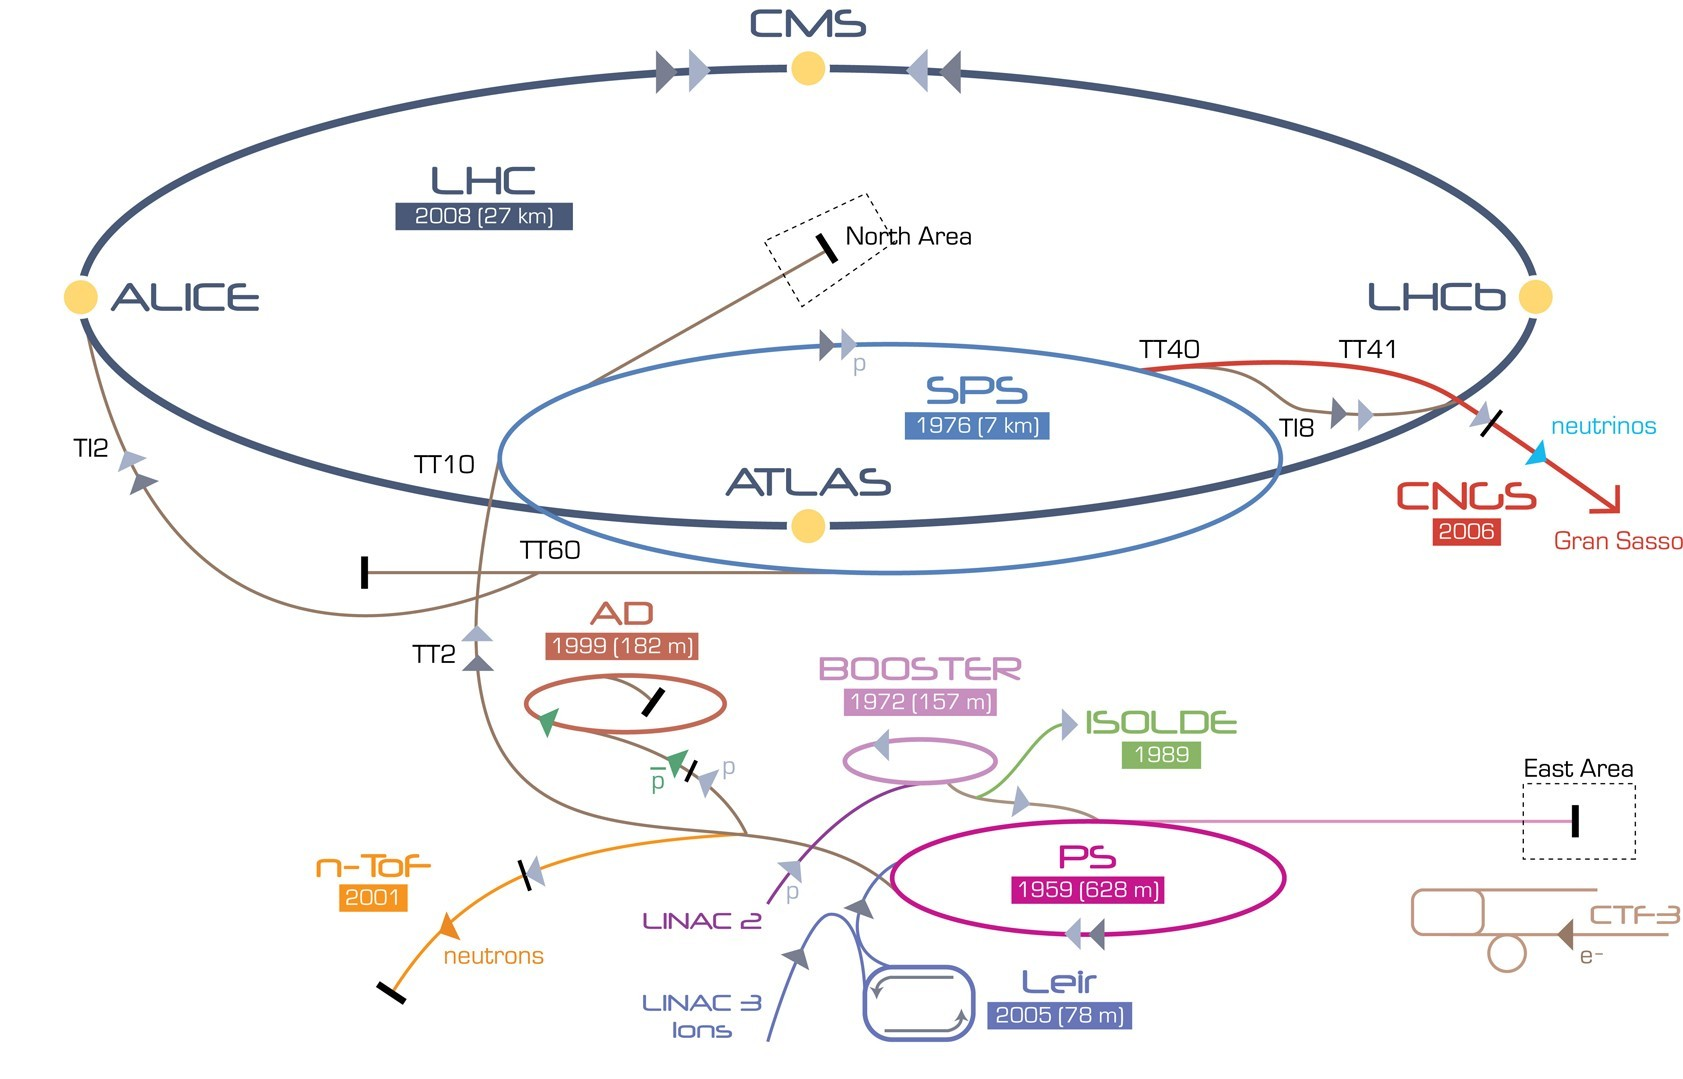
\includegraphics[width=\textwidth]{Figures/CERNAcceleratorComplex.jpg}
\caption{A full schematic of the full CERN accelerator complex.}
\end{figure}

\subsection{Pre-LHC accelerator complex}

The proton acceleration process begins by injecting Hydrogen ($H_2$) gas into a Duoplasmatron surrounded by an electric field, whereby the electrons become ionised through interactions with the free electrons from the cathode forming a plasma. This strips the electrons from the Hydroden leaving just the protons. The remaining protons are then linearly accelerated by the LINAC 2 accelerator, which uses radio frequency (RF) cavities to accelerate bunches of protons. By the end of this step the protons have reached an energy of up to 50 MeV and gained 5\% in mass. The next stage in the sequence sees the protons enter the Proton Synchroton Booster (PSB) which is composed of superimposed sychrotron rings which accelerate the received protons up to 1.4 GeV in 1.2 seconds before injection into the Proton Sychrotron (PS). The advantage of the Booster is that it allows the PS to accept over 100 times more protons by squeezing the proton bunches such that they have a much smaller cross-section. 

The PS is an essential component in the accelerator complex at CERN, where it accelerates either protons received from the PSB, or heavy ions from the Low Energy Ion Ring (LEIR). The apparatus first ran on the 24th of November 1959, and was, at that time, the worlds highest energy particle accelerator. Having a circumference of 628 metres, the PS comprises 277 conventional (room temperature) electromagnets, as well as 100 dipole magnets that serve to bend the beam around the ring. The PS accelerates protons, as well as other particles, up to 25 GeV in 3.2 s. The final stage of acceleration, before injection into the LHC, lies in the Super Proton Sychrotron (SPS). The SPS is the second largest of the CERN accelerators with a circumference of 7 kilometers, and provides beams for various experiments other than LHC: such as the NA61/SHINE and NA62 experiments, the COMPASS experiment, and the CNGS neutrino experiment. Protons are accelerated to 450 GeV  in 20 s within the SPS before injection into the LHC. Before the creation of LEP or the LHC the SPS was the primary collider at CERN, and in 1983 the collaboration won the Nobel prize for the discovery of the W and Z bosons in proton-antiproton collisions. The SPS comprises 1317 conventional electromagnets and 744 dipoles.

\subsection{Design of the LHC}

Two beams of protons are injected into the LHC and accelerated using RF cavities, one clockwise and the other counter-clockwise, taking roughly 20 minutes for each beam to reach the design energy of 7 TeV per beam. The two beams come into collision at four points around the $\sim27$ km ring where the collisions are recorded by the four detectors placed on the beam line. There are two all-purpose discovery detectors, namely CMS and ATLAS, studies of mesons by LHCb, and the study of heavy ions by the ALICE experiment. Because the tunnel in which the LHC is placed was designed for LEP it has an internal diameter of only 3.7 m, which is not large enough to install two separate beam pipes, and thus a design for a twin-bore magnet \cite{LHCStorageAccelerators}was created which would save space and cut costs substantially. Each beam is designed to hold 2808 bunches of protons with a bunch spacing of 50 ns. The protons are guided around the ring in a vacuum by superconducting electromagnets which are cooled to 1.9 K (-271.3$^\circ$) by using liquid helium. It consists of 1232 dipole magnets that are each 15 metres in length, and 392 quadrupole magnets that are 5-7 metres in length each which focus the beams. Before collisions can begin, a final shaping and cleaning of the beam takes place. Parameters for the LHC can be seen in Table \ref{tab-LHCparameters}.

\begin{table} \label{tab-LHCparameters}
\begin{center}
\begin{tabular}{|l|c|c|}
\hline
	\multicolumn{3}{|c|}{\textbf{LHC Parameters}} \\
\hline
	\textbf{Parameter} & \textbf{2012 Run} & \textbf{Design Value} \\
\hline	
	Beam Energy (TeV) & 4 & 7 \\
	Maximum number of bunches  & 1380 & 2808 \\
	Number of particles per bunch & $1.7\times 10^{11}$ & $1.15\times 10^{11}$ \\
	Bunch spacing (ns) & 50 & 25 \\
	Revolution frequency (kHz) & 11.245 & 11.245 \\
	Transverse beam size ($\mu$m) & 18.8 & 16.6 \\
	Peak luminosity (cm$^{-2}$s$^{-1}$) & $7.7\times 10^{33}$ & $10^{34}$ \\
	Stored beam energy (MJ) & 140 & 362 \\
	Normalised emittance at start of fill (mm mrad) & 2.5 & 3.75 \\
	$\beta^*$ in IP 1 and 5 (m) & 0.6 & 0.55 \\
\hline
\end{tabular}
\end{center}
\caption{LHC design parameters \cite{LHCDesignReport}.}
\end{table}


\subsection{Physics goals}

 There are many physics goals aimed to be achieved during the running of the LHC, but there are certain aims that are of a higher priority than others. One of the main focuses was the discovery of the Higgs boson and electroweak symmetry breaking, which was announced on the fourth of July 2012. This discovery was a triumph for the physics community in that it shed light on a fundamental building block of the universe which was theorised to exist some sixty years before its discovery. The theoretical physicist Peter Higgs subsequently won the Nobel prize for his work predicting the existence of a massive gauge boson in 1964. The Higgs a since been measured in various decay channels by both they ATLAS and CMS experiments with on-going studies aiming to measure properties of the boson, such as a the spin. Other physics goals include the search for supersymmetry, CP violation measurements, and studies of quark-gluon plasma using the ALICE experiment.  

\subsection{Luminosity at the LHC}

Due to the nature of individual detectors, not all require the same levels of delivered luminosity. For example, with CMS being an all-purpose discovery machine, the detector needs as much luminosity as possible, however an experiment like LHCb that measure mesons that are produced frequently and in a certain portion of the solid angle that the others use, less luminosity is required. The peak design luminosities for Run I and Run II are listed in Table \ref{tab-LHCparameters}. The instantaneous luminosity of a collider is calculated as

\begin{equation}
\mathcal{L}=f\frac{N_1N_2}{4\pi\sigma_x\sigma_y}
\end{equation}

where f is the collision frequency given by $f=u\times N_b$, the repetition frequency multiplied by the number of bunches in the beam, $N_{1,2}$ are the number of protons per bunch per beam, and $\sigma_{x,y}$ are the horizontal and vertical beam sizes at the interaction point (IP), respectively, and are defined as the product of the beams beta function and the proton beam emittance as shown in Equation \ref{eqn-beamsize}.

\begin{equation} \label{eqn-beamsize}
\sigma_{x,y}=\epsilon_{x,y}\beta_{x,y}
\end{equation}

The emittance of a beam describes the volume of the 6-dimensional phase space occupied by the proton bunch.

\subsection{Performance throughout run I}

Throughout Run I (2010 - 2013) the LHC operated with protons at beam energies of 3.5 and 4 TeV, where the beams consisted of single bunches and trains with different bunch spacing of 150 ns (2010), 75 ns (2011), and 50 ns (2011 and 2012). The performance of the LHC was much greater than initially expected at 50 ns, and culminated in the discovery of a $125 GeV/c^2$ Higgs boson in both the ATLAS \cite{ATLASHiggs} and CMS \cite{CMSHiggs} experiments. The use of 25 ns bunch spacing was only implemented in regards to electron-cloud scrubbing runs at the injection stage, and also for tests of future collisions with an upgraded LHC energy. One of the main focuses was to reduce the $\beta^*$ - the measure of how precisely the beam is focused at the interaction point. For ATLAS and CMS $\beta^*$ was lowered in steps from 3.5 mm in 2010 to 0.6 mm in 2012 by using tighter collimator settings. Other runs with mixed particle beams were also performed: such as proton-Pb, Pb-Pb, intermediate proton energy (1.38 TeV), and high beta.

For the 2012 run the default filling scheme introduced 1374 proton bunches per beam with 50 ns bunch spacing, giving ATLAS and CMS 1368 colliding bunches, 1262 in LHCb, and no colliding bunches in ALICE. The bunch intensity per beam peaked at $1.7 \times 10^{11}$ protons per bunch, which was then translated into a bunch intensity of $1.6 \times 10^{11}$ protons per bunch upon stabilisation of the beams. The transverse emittance remained constant throughout the year, despite moving to a different optical configuration with a lower transition energy. At the end of the runs the LHC had delivered an integrated luminosity of 23.3 fb$^{-1}$ to ATLAS and CMS, and over 2.1 fb$^{-1}$ to LHCb. The integrated and peak luminosity can be seen in Figure \ref{fig-LHClumi}, and the integrated luminosity recorded by CMS between 2011 ans 2013, and also compared to the total integrated luminosity delivered by the LHC, can be seen in Figure \ref{fig-CMSlumi}.

\newpage

\begin{figure} \label{fig-LHClumi}
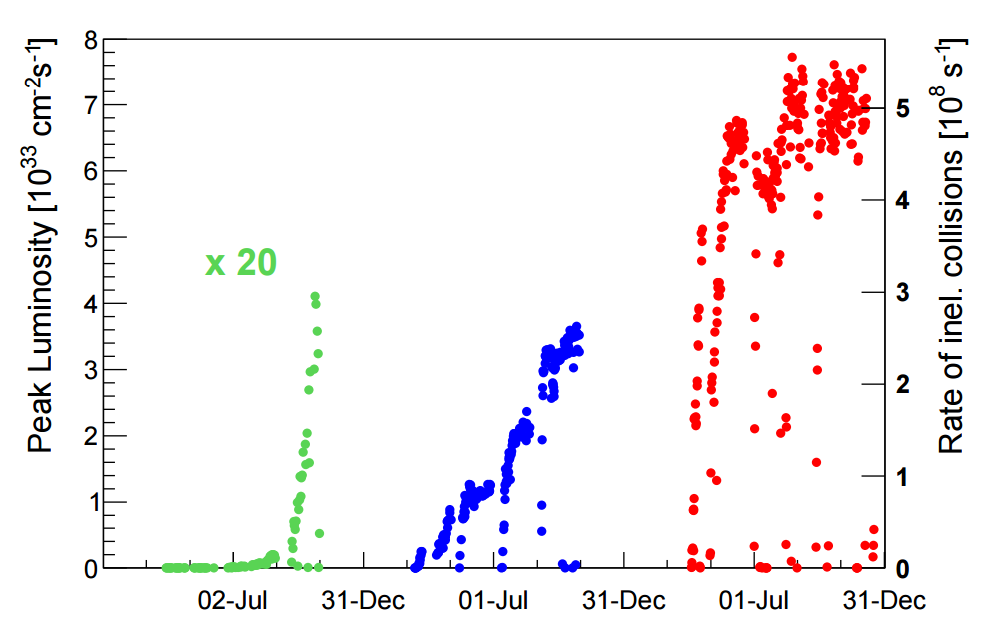
\includegraphics[width=0.5\textwidth]{Figures/LHClumi2.png}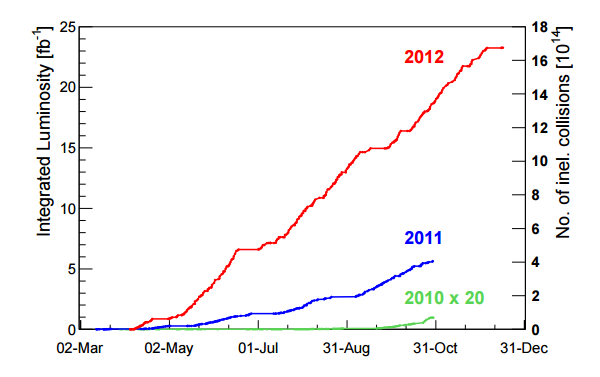
\includegraphics[width=0.5\textwidth]{Figures/LHClumi.png}
\caption{(Left) Peak and (right) integrated luminosity recorded by the LHC between 2010 and 2012 for proton operation. The 2010 luminosity values have been multiplied by a factor 20 \cite{LHClumi}.}
\end{figure}

\begin{figure} \label{fig-CMSlumi}
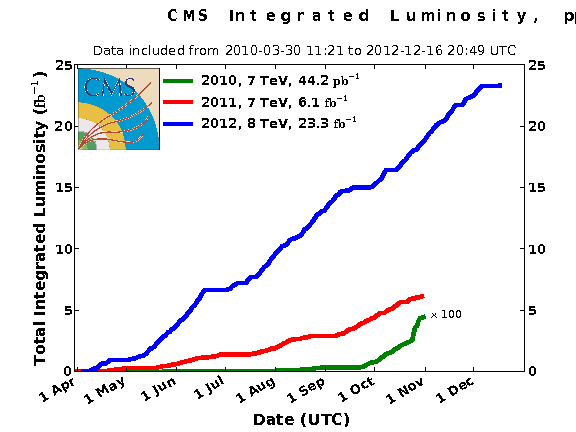
\includegraphics[width=0.5\textwidth]{Figures/IntLumi2.png}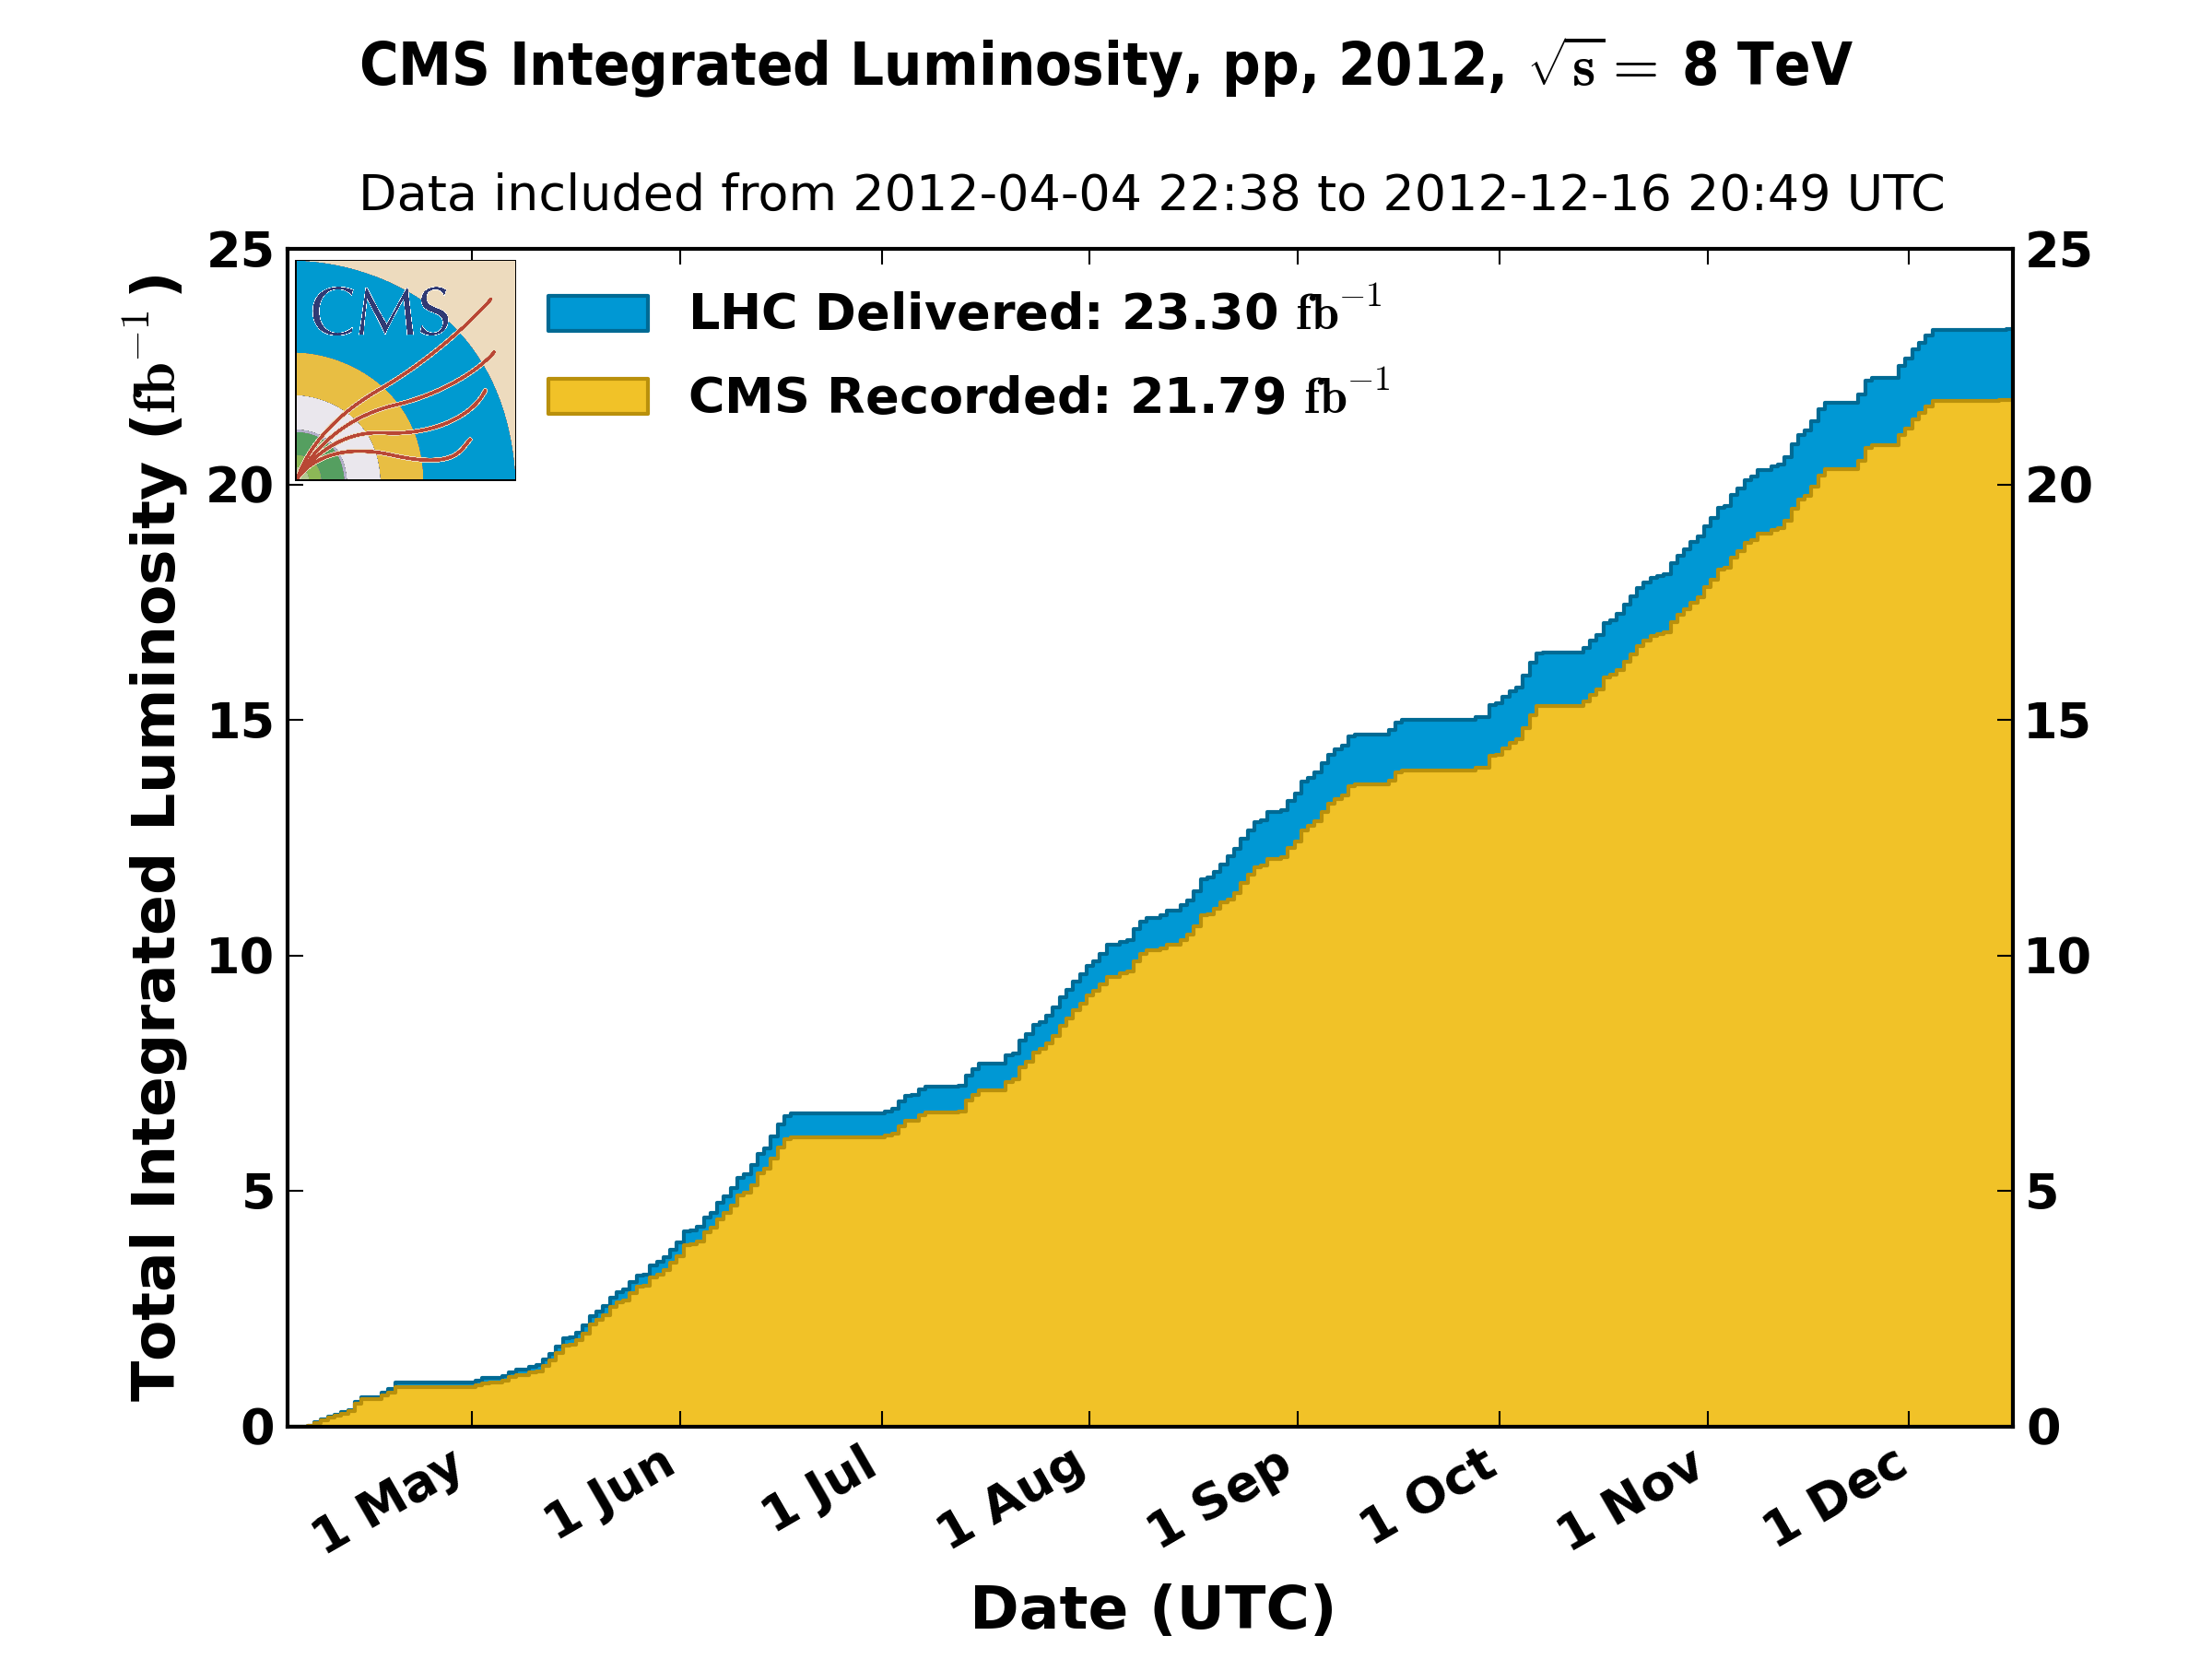
\includegraphics[width=0.5\textwidth]{Figures/CMSIntLumi.png}
\caption{Left: The accumulation of the integrated luminosity produced at the LHC vs time for runs in 2010, 2011, and 2012. The 2010 integrated luminosity is multiplied by 100 in order for it to be visible on the plot. Right: Total integrated luminosity vs time for the 2012 run in CMS and the LHC.}
\end{figure}

\newpage

\section{The CMS Detector} \label{sec-TheCMSDetector}

\begin{figure} [h!] \label{fig-CMSDetector}
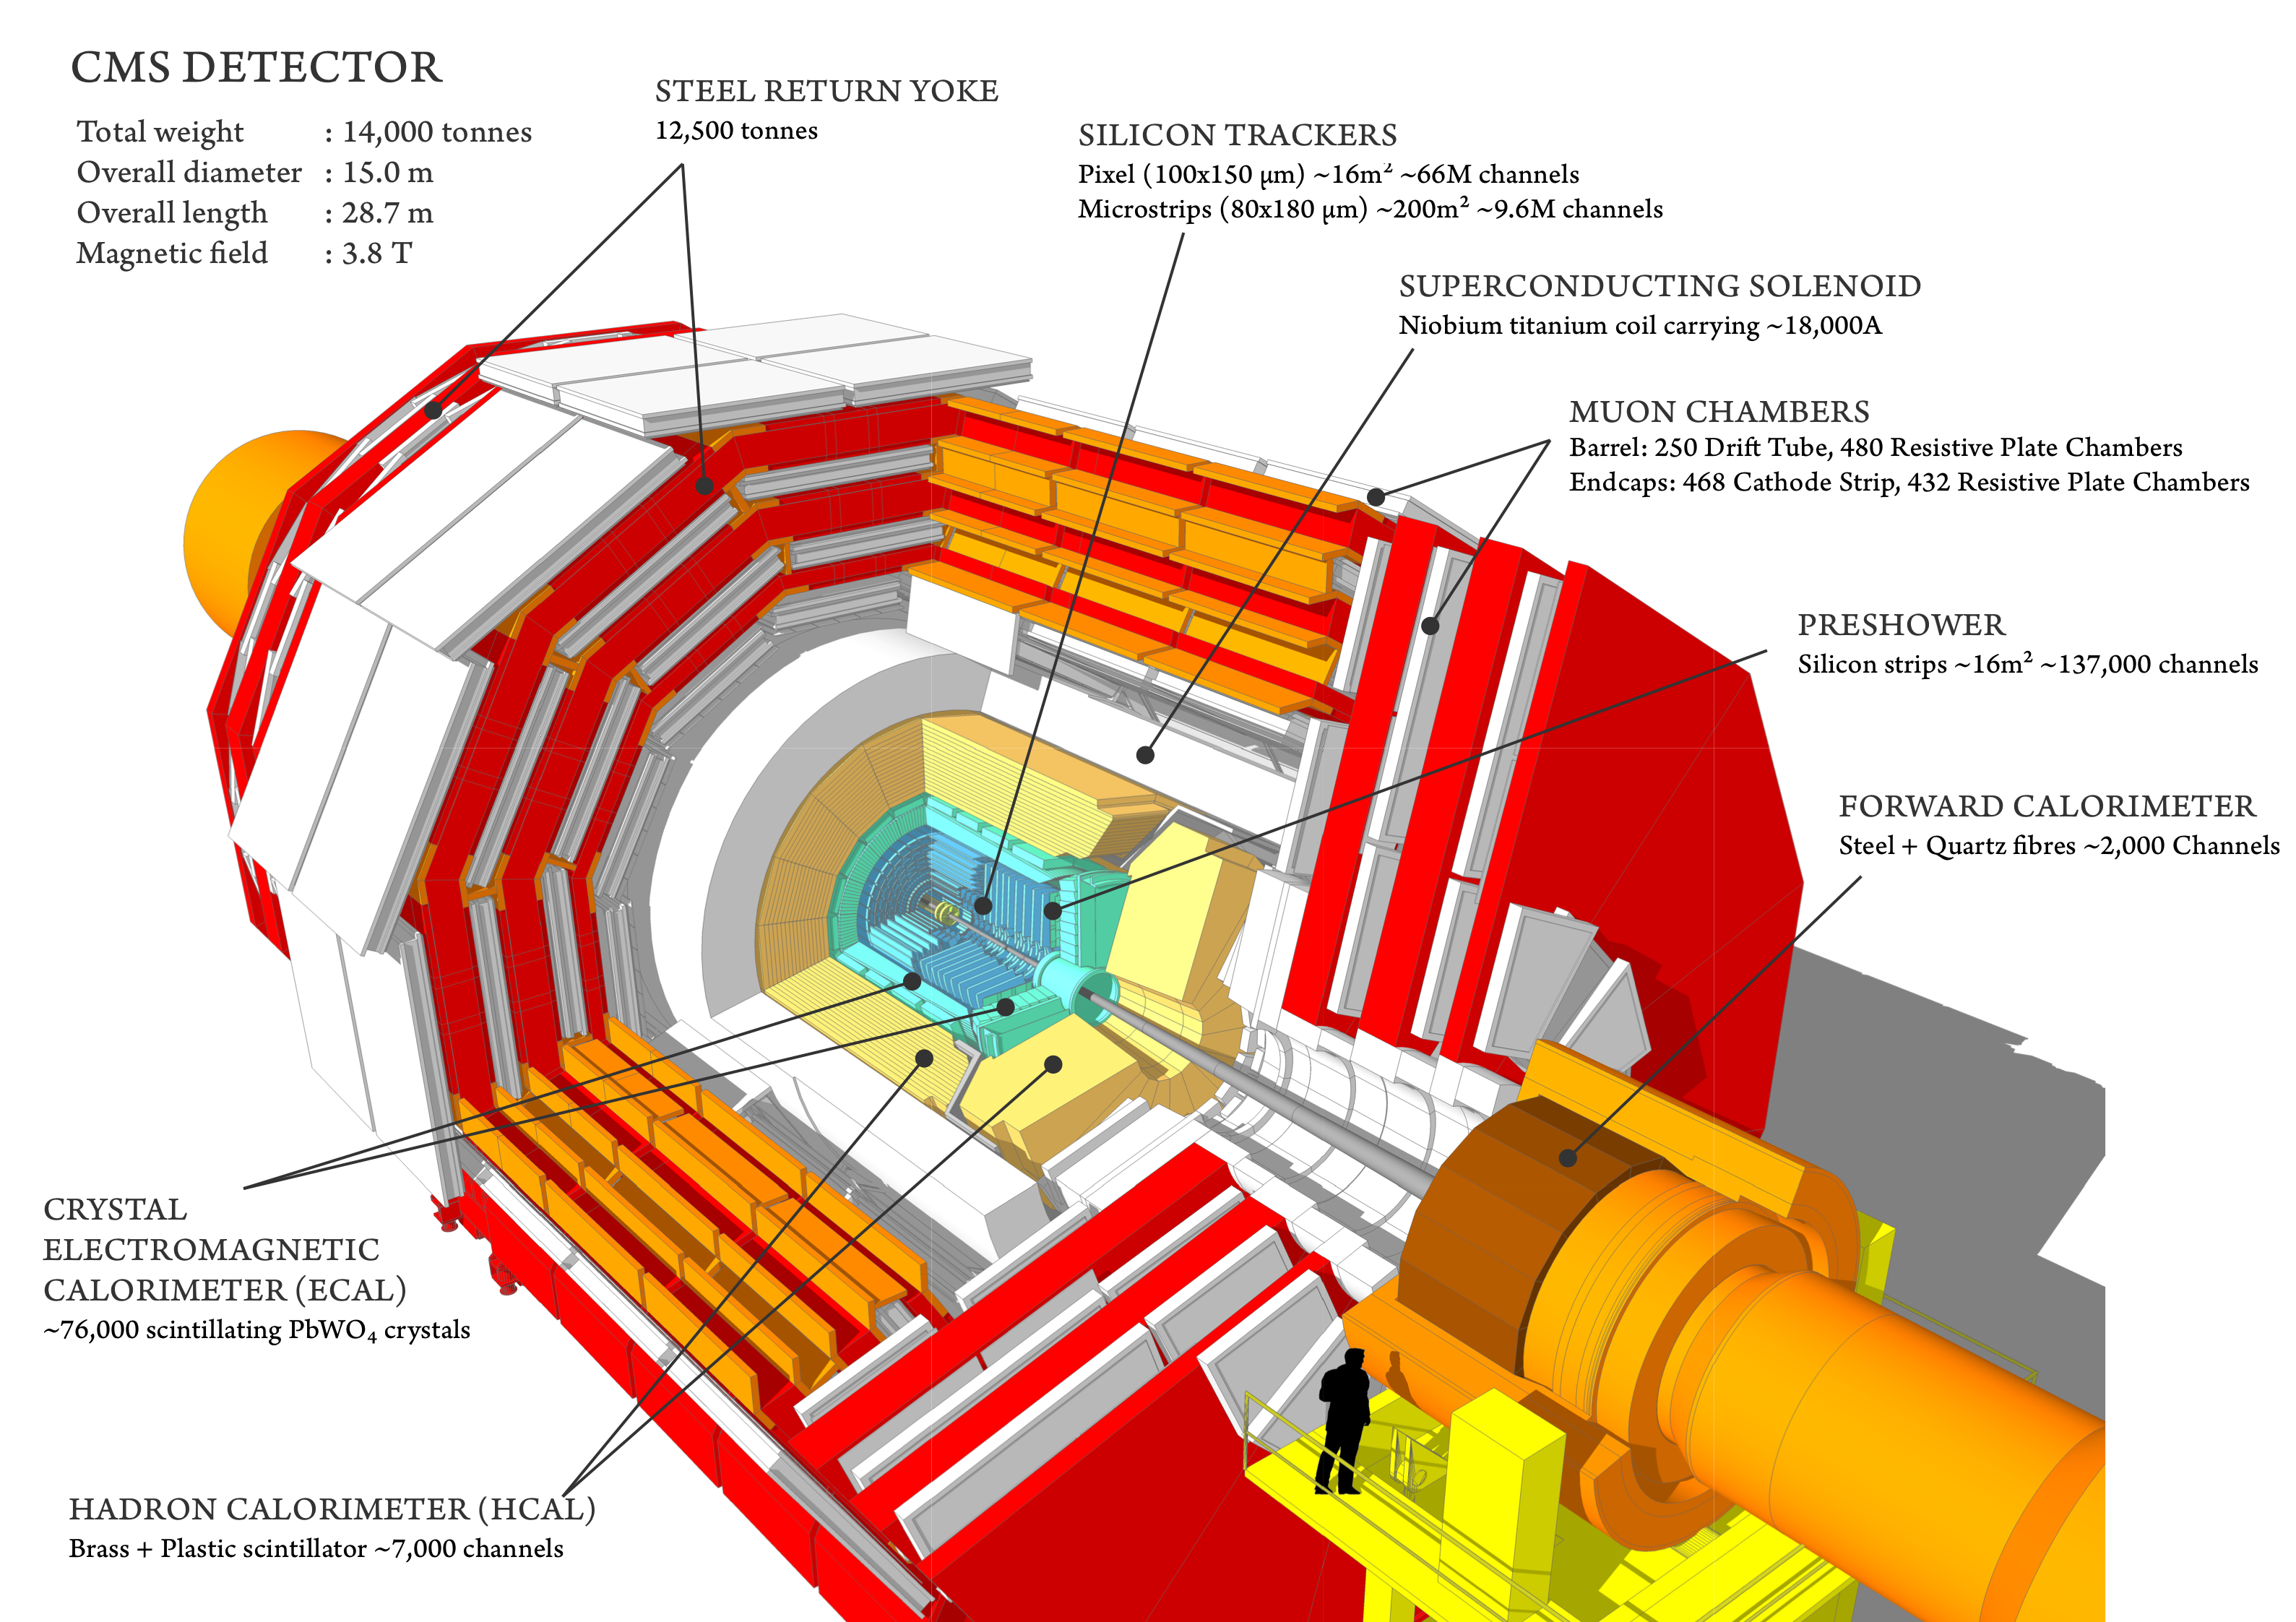
\includegraphics[width=\textwidth]{Figures/CMSDetector.png}
\caption{A cross-sectional view of the CMS detector.}
\end{figure}

The Compact Muon Solenoid (CMS) \cite{CMSexperiment} is one of the two all-purpose discovery machines located approximately 100 metres underground at point 5 (Cessy, France) on the LHC ring. Designed to cover the full solid angle, the hermetic detector is composed of multiple sub-detectors, described in detail in the following sections, designed to to perform precision particle detection and withstand extremely high doses of radiation. Unlike the other detectors that lie on the LHC ring CMS is designed with the purpose of precision measurements of Standard Model measurements and the discovery of physics beyond that of the Standard Model. The primary physics motivation for the construction of such a detector was to elucidate the nature of electroweak symmetry breaking of which the Higgs field was theorised to be responsible, which was proved correct in 2012 with the discovery of the quanta that propagates the Higgs field - the Higgs boson. Many theories predict to observe new physics at the TeV scale, and so CMS was designed with the intention to be able to withstand high energy and fluence of particles. Discovering physics beyond the Standard Model would pave the way for a potential unified theory. The detector weighs around 14,000 tonnes and has an overall length of 28.7 metres and diameter of 15 metres. A sectional view of the CMS detector labeling each sub-detector within is shown in Figure \ref{fig-CMSDetector}. CMS uses a right-handed coordinate system whereby the x-axis points towards the center of the LHC ring, the y-axis lies perpendicular to the beam, and the z-axis follows the direction of the beam anti-clockwise. The azimuthal angle, $\phi$, is measured from the x-axis in the xy plane where the radial component in this plane is define by r, and the polar angle $\theta$ in the rz plane. The pseudorapitiy is thus defined as 

\begin{equation}
\eta = -\ln \left(\tan\left(\frac{\theta}{2}\right)\right)
\end{equation}

and the momentum transverse to the beam is defined as p$_T$, and calculated using the x- and y-components. The transverse energy is defined as E$_T = E\sin\theta$. 

\section{Inner Tracking System} \label{sec-InnerTrackingSystem}

The first sub-detector system located closest to the beam is the Inner Tracking System. The Inner Tracking System is composed of several modules that work in conjunction to provide precise and efficient measurements of the trajectories of charged particles resulting from the beam collisions, as well as a precision reconstruction of secondary vertices, whereby the product from the LHC beam collision decays. The tracker is completely hermetic around the interaction point (IP) of the beam-line, is 5.8 m in length, and has a diameter of 2.5 m. In order to reconstruct particle tracks momentum measurements must be made. To do this the tracker works in combination with the CMS Superconducting Solenoid (Section \ref{sec-SuperconductingSolenoid}) with a magnetic field at 4 T. 

Due to the high flux of the LHC at design luminosity the inner tracker will receive around 1000 particles per bunch crossing with around 20 primary vertices per collision, therefore the tracker was designed to operate with a high granularity and fast response time such that trajectories can be precisely identified and associated with the correct bunch crossing. Several challenges arise upon implementation of such technology: the requirement of high power density to the on-detector electronics means that sufficient cooling must be used throughout, which then conflicts with the ideology of keeping material to a minimum to prevent effects such as multiple scattering, bremsstrahlung, photon conversion, and nuclear scattering. Another challenge presents itself in the form of radiation damage to the tracking system due to the large flux of high energy particles over time. The requirements for a high granularity detector using minimum material that can run over a period of roughly 10 years whilst remaining radiation hard lead to a final design entirely based on silicon detector technology. 

Shown in Figure \ref{fig-Tracker}, the Inner Tracking System is composed of a pixel detector with a radii of between 4.4 cm and 10.2 cm, and a silicon strip tracker which in composed of 10 barrel detection layers reaching a radius of 1.1 m. In order to make tracking system completely hermetic the barrel detectors are surrounded by endcaps composed of 2 disks in the pixel detector and 3 plus 9 disks of silicon strip tracker, thus extending the acceptance, $A$, of the tracker up to a pseudorapidity of $|\eta| < 2.5$.  Each individual pixel station covers a region of $100\times150$ $\mu$m$^2$ in the $r-\phi$ and $z$ coordinate system, respectively, and is driven by the desired impact parameter resolution. In total the pixel detector contains 66 million pixels, corresponding to an active area of 1 m$^2$.

\begin{figure} [h!] \label{fig-Tracker}
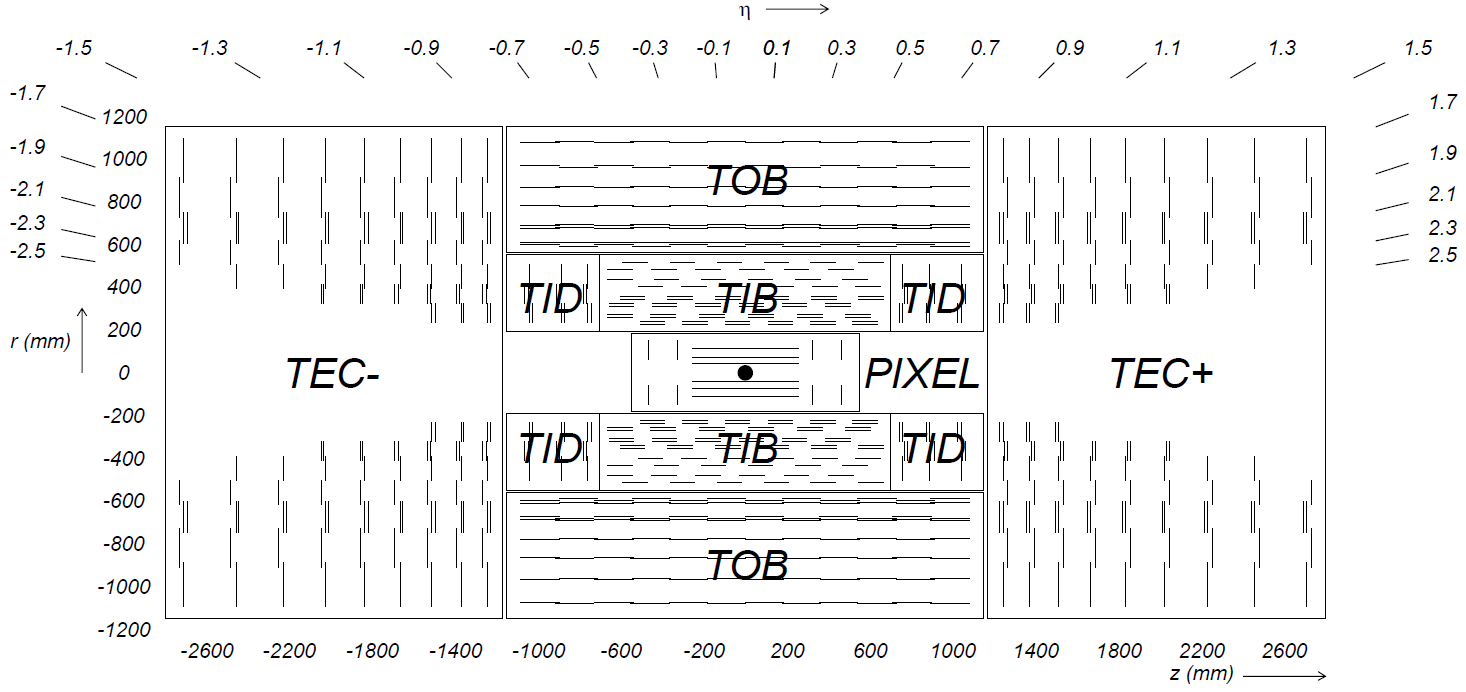
\includegraphics[width=\textwidth]{Figures/Tracker.png}
\caption{The sub-detectors of the CMS silicon tracker system: TOB=outer barrel, TIB=inner barrel, TID=inner disc, TEC=endcaps, PIXEL=pixeldetector. Each line represents a detector module. Double lines indicate back-to-back modules which deliver stereo hits. \cite{CMSexperiment}.}
\end{figure}

The sensor elements in the silicon strip tracker system are single sided p-on-n type silicon micro-strip sensors \cite{SiliconStripSensors1,SiliconStripSensors2}. The Tracker Inner Barrel (TIB) and Disks (TID), where the particle flux is smaller, extends to a radius of between 20 cm $< r <$ 55 cm, and has a typical cell size of 10 cm $\times 80 \mu$m$^2$, strip thickness of $320 \mu$m, and an occupancy of $\sim2-3\%$ per strip per bunch crossing. The outer layer of the silicon strip tracker ranges from 55 cm $< r <$ 110 cm and $\sim500 \mu$m thick, but with a cell size of 25 cm $\times$ 180 $\mu$m due to lower levels of radiation in the outer region. The TIB and TID are surrounded by the Tracker Outer Barrel (TOB) which has an outer radius of 116 cm and comprises 6 barrel layers of 500 $\mu$m thickness micro-strip sensors and strip patches of 183 $\mu$m on the first 4 layers and 122 $\mu$m on the 5th and 6th layers. Beyond the range of the TOB lies the Tracker EndCaps (TEC+ and TEC-, where the sign represents the location of the endcap along the z-axis) to provide complete coverage. The TECs cover the region 124 cm $<|z|<$ 282 cm and 22.5 cm $<|r|<$ 113.5 cm and is composed of 9 disks each consisting of 7 rings of silicon micro-strip detectors, 320 $\mu$m thick on the inner 4 rings, 500 $\mu$m thick on rings 5-7) with radial strips of 97 $\mu$m to 184 $\mu$m average pitch. Therefore, they provide up to 9 $\phi$ measurements per trajectory.

\subsection{Tracker performance in Run I} \label{subsec-TrackerPerformance}

Over the Run I period, from 2010 to 2013, the LHC delivered around 6 fb$^{-1}$ at 7 TeV and 23.3 fb$^{-1}$ at 8 TeV (Figure \ref{fig-LHClumi}), out of this approximately 93\% was recorded by CMS. The CMS tracker was responsible for roughly one third of the lost data due to the high voltage only being ramped up once stable beams are reached. By the end of Run I approximately 2.3\% of the tracker barrel and 7.2\% of the endcap modules were inactive associated with faulty wire-bonds or poor connections. During this period around 2.5\% of the strip detector became inactive because of short-circuits in the control rings and HV lines, or due to faulty optical communications. Maintenance and repairs began upon shutdown of the LHC, and CMS was able to salvage up to 1.5\% of the pixel barrel, up to 0.5\% of the pixel endcap modules, and up to 1\% of the strip detectors \cite{TrackerPerformance}.

In order to process the data prior to track reconstruction the hit efficiency must be measured, the points at which a charged particle traversed each layer of the inner tracker. After track reconstruction the efficiency is calculated as the fraction of particles that are expected to pass through the fiducial regions of the sensors in a layer of the detector in which matching hits are found. For the strip detectors a hit is considered to be a hit if the energy deposit is found in the module in which it was expected to be observed. For efficient reconstruction of tracks knowledge of the position of each module in three-dimensional space is required. Distortions and movements of the inner tracker modules were monitored using cosmic ray data and collision tracks by measuring the distance between expected and observed track trajectories. Distortions in tracking lead to biases in the reconstructed track curvature, and were studied using the reconstructed mass of $Z \to \mu\mu$ events as a function of the positive muon's azimuthal angle. The muon reconstruction efficiency can be seen in Figure \ref{fig-MuonReconstructionEfficiency}.

\begin{figure} \label{fig-MuonReconstructionEfficiency}
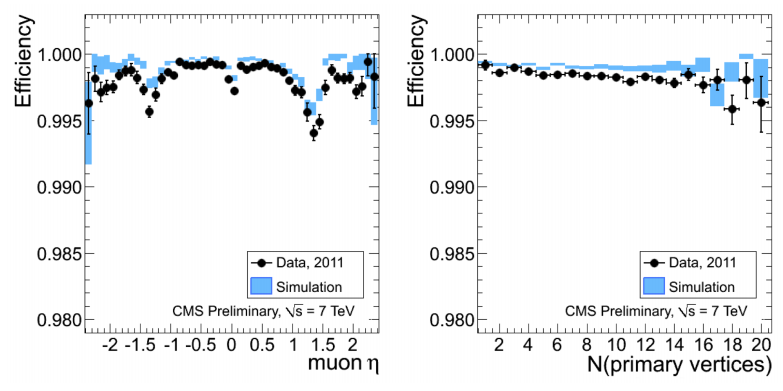
\includegraphics[width=\textwidth]{Figures/MuonReconstructionEfficiency.png}
\caption{Muon reconstruction efficiency in thee tracker as functions of pseudorapidity (left) and the number
of proton-proton interaction vertices (right) \cite{TrackingResults}.}
\end{figure}

\begin{figure} \label{fig-PVResolution}
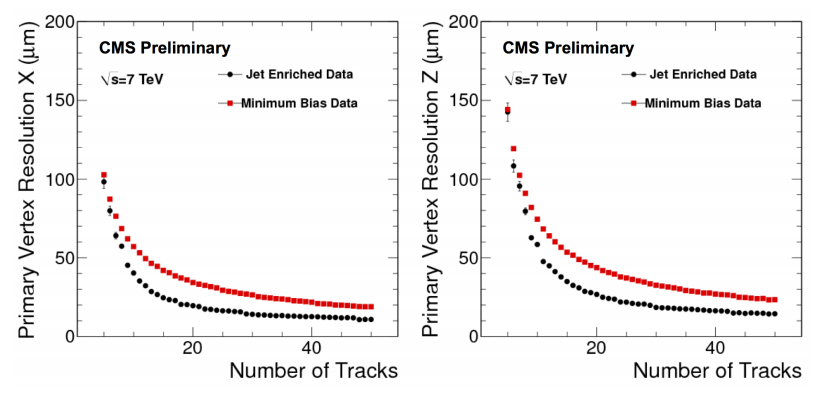
\includegraphics[width=\textwidth]{Figures/PVResolution.png}
\caption{Primary vertex resolution in the transverse plane (left) and along the beam-line (right) as functions
of the number of tracks attached to the vertex \cite{TrackingResults}.}
\end{figure}

The CMS tracking software relies on an iterative procedure to measure hits in a high particle occupancy environment. Earlier steps of the tracking process search for tracks with higher p$_T$ due to the more obvious nature of the tracks, which include a smaller impact parameter, and greater number of measured hits in each layer of the tracker. By selecting more obvious processes first, the reconstruction becomes easier as it has fewer events to deal with. Track reconstruction efficiency is measured by using the tag and probe method in $Z \to \mu\mu$ events \cite{TrackingResults}. The tracking efficiency is then defined as the number of probes observed to have matching tracks within the tracker and is a function of the number of primary vertices and the pseudorapidity of the tracks and can be seen in Figure \ref{fig-PVResolution}. LHC proton-proton events are reconstructed by firstly identifying the tracks, then grouping in accordance with their primary vertex, and finally fitting to the position of each vertex.  

One of the long term damaging effects of high luminosity collisions is radiation damage. Radiation damage in the silicon was monitored throughout Run I and tested by performing special runs where the bias voltage was increased in steps from 0 to the operational voltages. Results showed that the hit efficiency decreased with irradiation at first, then increased with changes in the effective doping \cite{Doping}. Due to collisions not being completely aligned at the centre of the detector, even irradiation of the modules is seen in the azimuthal direction.

Overall, the CMS tracker has performed exceptionally throughout the Run I three-year period with regards to detector reliability and tracking. The tracker was able to overcome a major problem of high pile-up and reconstruct tracks with excellent efficiency. Less than 3\% of the tracker became inactive throughout the entire run, and less than 5\% of the delivered luminosity was lost through the tracker.    
 
\section{Electromagnetic Calorimeter} \label{sec-ElectromagneticCalorimeter}

\subsection{Overview} \label{subsec-ECALOverview}

Directly after the Inner Tracking System, the second stage of particle identification and reconstruction comes in the form of the Electromagnetic Calorimeter (ECAL). The ECAL serves to stop electromagnetic particles, namely electrons and photons, and measure the energy deposited in the detector. These particles are identified and reconstructed using signatures such as charge, shower shape, and isolation. When an electron passes through the ECAL it showers via bremsstrahlung. Radiation losses due to bremsstrahlung scale with mass as m$^{-4}$ (m$^{-6}$) when a charged particle travels perpendicular (parallel) to an electric field, and thus heavier electromagnetic particles are less likely to produce a shower. It is possible to differentiate between electrons and positrons by the curvature produced from the Superconducting Solenoid. Photons are neutrally charged and thus do not bend via the magnet, however they produce a shower of electron-positron pairs which can then be measured. The photon shower shape, known as $\sigma_{i\eta i\eta}$, is a prominent variable in this analysis and will be described in detail in Section \ref{sec-}.  

A key component that drove the design of the ECAL is the decay channel $H \to \gamma\gamma$. At the time of design, the Higgs had not been discovered and thus the mass was not known, however it was known that the aforementioned decay mode was sensitive to a low mass Higgs, $m_H<150$ GeV. Although the branching ratio of the decay is small ($\simeq0.002$), the signature is clean and is a narrow resonance of two high E$_T$ photons over a non resonant background \cite{HiggsProposal}. In order to discover the Higgs the detector needed to have a powerful invariant mass resolution and background rejection, translating into a need for extremely efficient photon and electron identification, along with a high position and energy resolution. 

\subsection{Composition of the ECAL} \label{subsec-ECALComposition}

The CMS ECAL is a is a hermetic, homogeneous fine-grained lead tungstate (PbWO$_4$) crystal calorimeter \cite{ECAL}, shown in Figure \ref{fig-ECAL}. The PbWO$_4$ crystals are extremely dense  ($\delta=8.28$ g/cm$^3$), thus providing excellent performance and compactness, and thus fit within the Superconducting Solenoid magnet volume. The crystals were designed with an extremely small radiation length, $X_0=0.85$ cm, and small Moli\`{e}re radius, $R_M=2.19$ cm. The decision to use a homogeneous medium was chosen because of the ability to obtain a greater energy resolution by minimizing sampling fluctuations \cite{ECAL}. 

\begin{figure} [h!] \label{fig-ECAL}
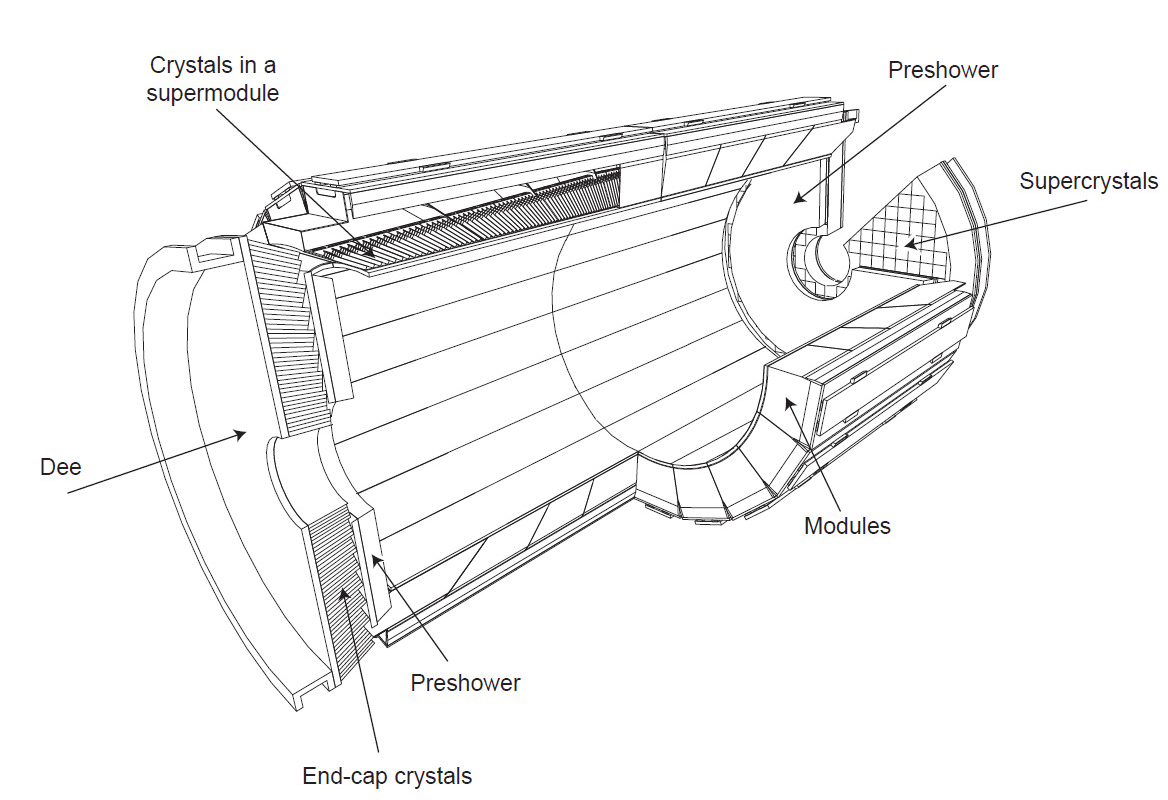
\includegraphics[width=\textwidth]{Figures/ECAL.png}
\caption{Geometric view of one quarter of the ECAL (top). Layout of the CMS electromagnetic calorimeter presenting the arrangement of crystal modules, supermodules, endcaps and the preshower in front (bottom) \cite{CMSexperiment}.}
\end{figure}

There are 75,848 within the ECAL, and are arranged into a barrel section (EB), covering a pseudorapidity rang of $|\eta|<1.4442$, which is then surrounded by endcaps and thus extending the pseudorapidity range to $|\eta|<3.0$. The length of the crystals within the barrel are 230 mm and 220 mm in the endcap regions, which corresponds to $\sim26$ (EB) and $\sim25$ (EE) radiation lengths. The crystals are projective and also slightly off-pointing in position, $\sim3^\circ$ with respect to the IP. This configuration provides a full coverage and ensures that there are no cracks in the calorimetry that are aligned with particle trajectories. Within the barrel there is no longitudinal segmentation, and therefore the angle at which a photon is measured relies on the reconstructed PV from the silicon tracker. EB crystals are $2.2\times2.2$ cms$^2$ on the front face, and $2.86\times2.86$ cm$^2$ in the endcaps, giving rise to a total crystal volume of 11 m$^3$ and a weight of 92 t.

The barrel crystals are arranged into 36 supermodules (or superclusters), each containing 1,700 crystals, whereas the endcaps are arranged into two D-shaped segments comprising 3,662 crystals each. The final section of the ECAL is the pre-shower detector system (ES) placed directly in front of the endcaps at $1.65<|\eta|<2.6$ and can be visualised in Figure \ref{fig-ECALRapidity}. The ES is composed of 4,288 sensors, 137,216 silicon strip sensors, each $1.90\times61$ mm$^2$ with x-y view, and has a total of $\sim3$ radiation lengths. The purpose of the ES is provide improved separation of photons to $\pi^0$s.

\begin{figure}\label{fig-ECALRapidity}
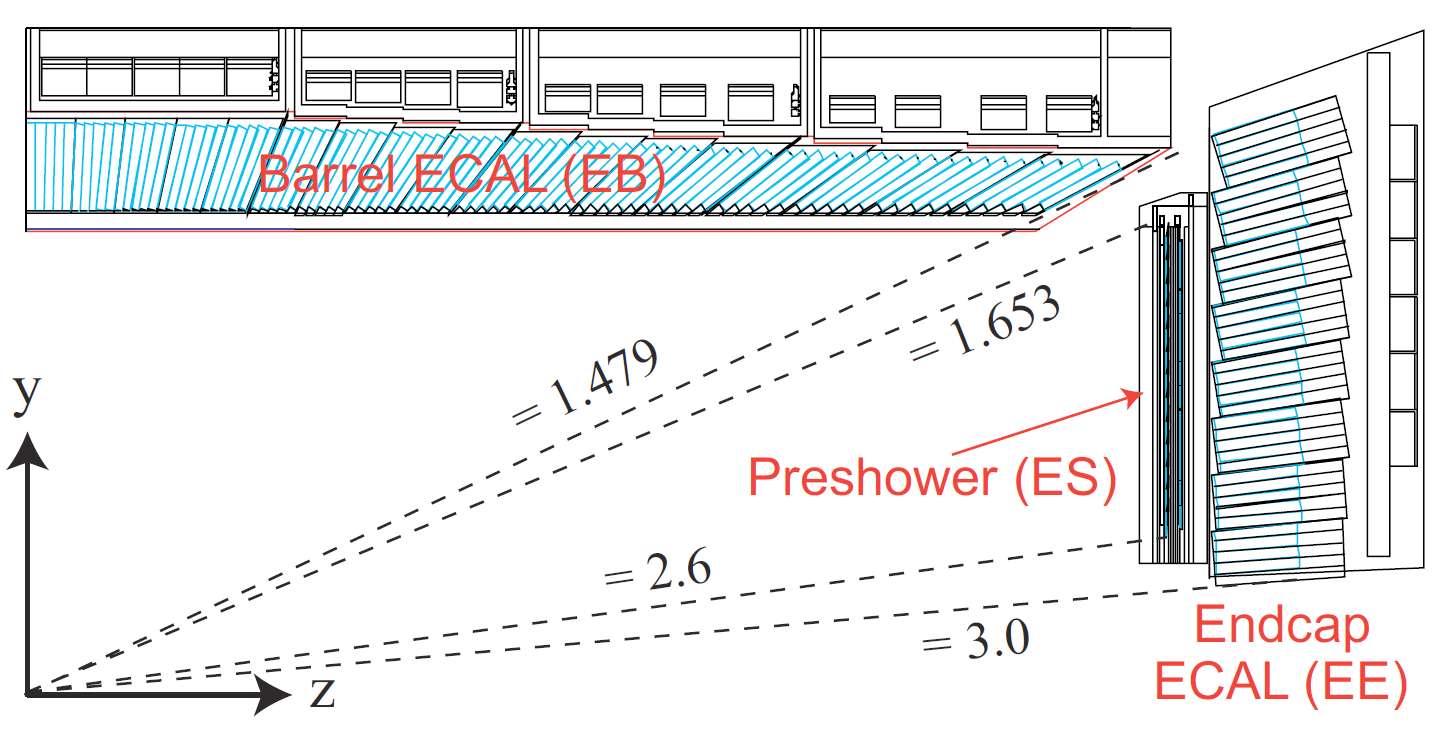
\includegraphics[width=\textwidth]{Figures/ECALRapidity.png}
\caption{Geometric view of one quarter of the ECAL (top). Layout of the CMS electromagnetic calorimeter presenting the arrangement of crystal modules, supermodules, endcaps and the preshower in front (bottom) \cite{CMSexperiment}.}
\end{figure}

\subsection{Photodetectors} \label{subsec-Photodetectors}

The light read-out system for the barrel crystals comes in the form of Hamamatsu avalanche photodiodes (APD). There are two APDs for each crystal which are read in parallel, each measuring $5\times5$ mm$^2$ with a quantum efficiency (QE) of 75\%. The gain is set at $\sim50$ and they are insensitive to the 4 T magnetic field from the Superconducting Solenoid. The endcap crystals scintillation light is read out by vacuum photo-triodes (VPT), each with an area of 280 mm$^2$ with a 20\% QE and gain of $\sim10$. The barrel APDs are temperature sensitive ($\frac{1}{E}\frac{dE}{dT}\sim-2.3\%C^{-1}$) whereas the VPT sensitivity to temperature is assumed to be negligible relative to that of the crystals.  

\subsection{Performance of the ECAL throughout Run I} \label{subsec-ECALPerformance}

The energy resolution, $\frac{\sigma_E}{E}$ of the ECAL crystals can be parameterised by

\begin{equation}
\left(\frac{\sigma_E}{E}\right)^2 = \left(\frac{A}{\sqrt{E}}\right)^2 + \left(\frac{B}{E}\right)^2 + C^2
\end{equation}

where A and B are the stochastic term for scintillation showers and noise term due to read-out electronics and PMTs, respectively. C is a constant term which is a direct measure of the performance of the PbWO$_4$ crystals. 

\begin{figure} \label{fig-}
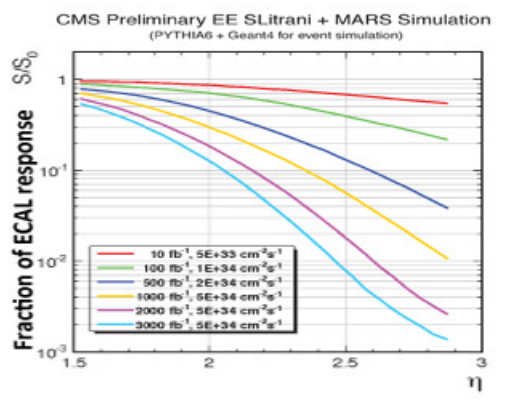
\includegraphics[width=0.48\textwidth]{Figures/EEFractionalResponse.png}
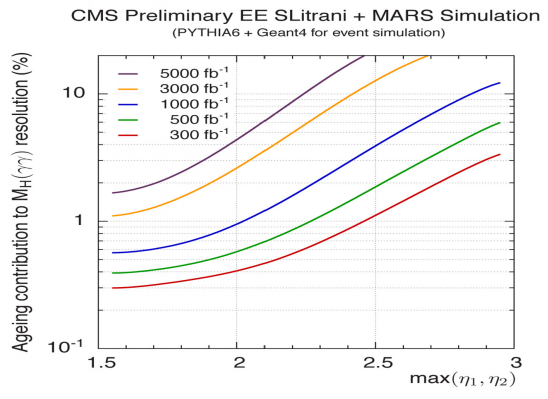
\includegraphics[width=0.52\textwidth]{Figures/EEResolutionDeterioration.png}
\caption{Simulation of fractional response from EE as a function of $\eta$, for different integrated luminosities. Right: Deterioration of the energy resolution in EE as a function of $\eta$, for different integrated luminosities \cite{ECALPerformance}.}
\end{figure}

\section{Hadron Calorimeter} \label{sec-HadronCalorimeter}

\section{Superconducting Solenoid} \label{sec-SuperconductingSolenoid}

The CMS Superconducting Solenoid, shown in Figure \ref{fig-SuperconductingSolenoid}, is the most powerful magnet in the world, 100,000 times stronger than the Earth's magnetic field and stores enough energy to melt 16 tonnes of gold, and the most essential feature of the detector. In order to achieve a good momentum resolution in such a detector, without making tight cuts on muon chamber resolution and alignment, a powerful magnetic field was chosen. A large bending power can be achieved by a modestly sized solenoid, as long as it is a high-field superconducting one, due to the bending beginning at the primary vertex. The requirement for the bending power of the solenoid is dictated by the narrow states decaying into muons, and by the unambiguous determination of the sign for muons with a momentum of around 1 TeV/c. In order to obtain a precision measurement, a momentum resolution of $\Delta p/p\approx10\%$ at p = 1 TeV/c. A suitable length to radius ratio is required to obtain a good momentum resolution in the forward region, and can be seen in the parameters listed in Table \ref{tab-SolenoidParameters} \cite{PTDR2}. 

\begin{table} \label{tab-SolenoidParameters}
\begin{center}
\begin{tabular}{|l|c|}
\hline
	\multicolumn{2}{|c|}{\textbf{Superconducting Solenoid Parameters}} \\
\hline
	\textbf{Parameter} & \textbf{Value} \\
\hline
	Field (T) & 4 \\
	Length (m) & 12.9 \\
	Weight (t) & 250 \\
	Inner bore (m) & 5.9 \\
	Current (kA) & 19.5 \\
	Number of turns & 2168 \\
	Stored energy (GJ) & 2.7 \\
	Hoop stress (atm) & 64 \\
\hline
\end{tabular}	
\caption{Parameters of the LHC superconducting solenoid \cite{MagneticField}.}
\end{center}
\end{table}

Approaching 13 m in length, and 6 m in diameter, the solid mass weights approximately 250 t at an operating temperature of $-268.5^\circ C$ -- a degree warmer than outer space. Originally designed to run with a uniform magnetic field of 4 T within the 5.9 m bore, the eventual operating level was set to 3.8 T in order to increase the lifetime. Such a magnetic field requires a return yoke, which can be viewed in the CMS schematic in Figure \ref{fig-CMSDetector}, of which the return field is large enough to saturate 1.5 m of iron and weighs 12,500 t. This allows four muon stations to be integrated within the return yoke, ensuring robustness and full geometric coverage. The magnet and return yoke use almost twice as much iron as the Eiffel Tower.

\begin{figure} \label{fig-SuperconductingSolenoid}
\begin{center}
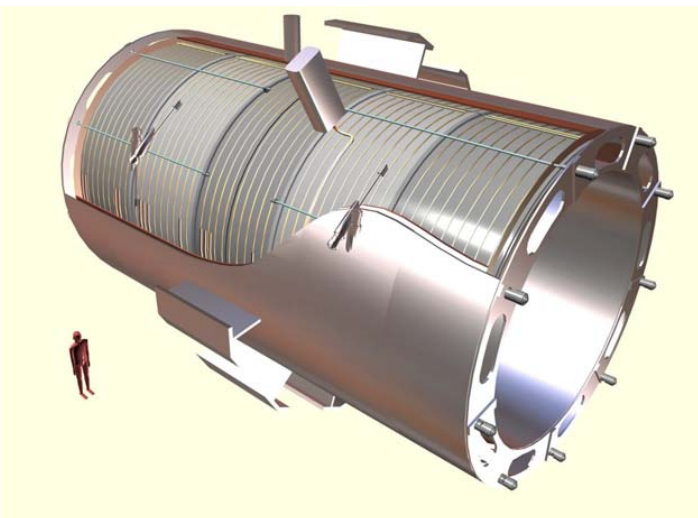
\includegraphics[scale=0.5]{Figures/SuperconductingSolenoid.png}
\caption{ General artistic view of the 5 modules composing the cold mass inside the cryostat, with details of the supporting system (vertical, radial and longitudinal tie rods) \cite{CMSexperiment}.}
\end{center}
\end{figure}


\section{Muon System} \label{sec-MuonSystem}

CSCs
RPCs
DTs

\begin{figure}\label{fig-CMSLongitudinalView}
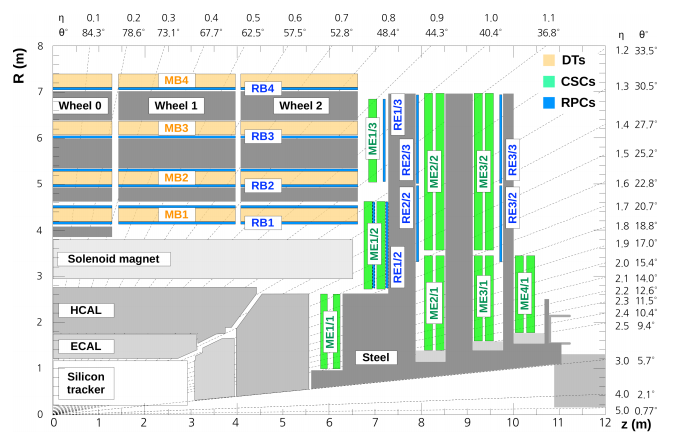
\includegraphics[width=\textwidth]{Figures/CMSLongitudinalView.png}
\caption{Layout of one quadrant of CMS. The figure shows the four DT stations in the barrel (MB1-MB4, yellow), the four CSC stations in the endcap (ME1-ME4, green), and the RPC stations (RB1-RB4 and RE1-RE3) \cite{CMSexperiment}.}
\end{figure}

\section{Trigger} \label{sec-Trigger}

At design energy, the total proton-proton cross-section is expected to be approximately 100 mb, and should therefore observe around $10^9$ events/s. This extremely high rate of events leads to numerous experimental and technological challenges, namely the read-out and triggering systems. There will be roughly 20 inelastic events that will be superimposed onto events that are triggered on, known as pile-up (PU). 

\section{Particle Reconstruction} \label{sec-ParticleReconstruction}

\subsection{Electron identification}

\subsection{Muon reconstruction}

\subsection{Jet reconstruction}

\subsubsection{Jet energy corrections}

\subsubsection{Particle flow jet identification}

\section{Computing}

\subsection{Event Data Model}

\subsection{Analysis Software}

\section{Monte Carlo Simulation}

\begin{sidewaystable} \label{tab-MCSamples}
\begin{center}

\begin{tabular}{|l| p{12.5cm} |c|p{2cm}|}
\hline
	\textbf{Process} & \textbf{Dataset} & \textbf{$\sigma$ (pb)} & \textbf{Number of events} \\
\hline
	$t\bar{t}+\gamma (2\to5)$ & /LHE2EDM\_WHIZARD\_2to5\_ttA/htholen-FULLSIM\_STEP2\_WHIZARD\_2to5\_ttA-da43ae45efb6a7c35e17aad82de2e2cd/USER & 1.8 & 1074860 \\
	$t\bar{t}+\gamma (2\to7)$ & /TTGamma\_TuneZ2star\_8TeV-madgraph-tauola/Summer12\_DR53X-PU\_RD1\_START53\_V7N-v1/AODSIM & 1.8 & 916500\\ 
\hline	
	$t\bar{t}(Leptonic)$ & /TTJets\_FullLeptMGDecays\_8TeV-madgraph/Summer12\_DR53X-PU\_S10\_START53\_V7A-v2/AODSIM & 245.8 & 12119013\\
	$t\bar{t}(Hadronic)$ & /TTJets\_HadronicMGDecays\_8TeV-madgraph/Summer12\_DR53X-PU\_S10\_START53\_V7A\_ext-v1/AODSIM & 245.8 & 31223821\\
	$t\bar{t}(Semileptonic)$ & /TTJets\_SemiLeptMGDecays\_8TeV-madgraph/Summer12\_DR53X-PU\_S10\_START53\_V7A\_ext-v1/AODSIM & 245.8 & 25424818\\
	$t\bar{t}(Inclusive)$ & /TTJets\_MassiveBinDECAY\_TuneZ2star\_8TeV-madgraph-tauola/Summer12\_DR53X-PU\_S10\_START53\_V7C-v1/AODSIM & 245.8 & 6923652\\
\hline	
	Drell-Yann, $10 < m\_{ll} < 50$ & /DYJetsToLL\_M-10To50\_TuneZ2Star\_8TeV-madgraph/Summer12\_DR53X-PU\_S10\_START53\_V7A-v1/AODSIM & 11050.0 & 37835275\\
	Drell-Yann, $m\_{ll} > 50$ & /DYJetsToLL\_M-50\_TuneZ2Star\_8TeV-madgraph-tarball/Summer12\_DR53X-PU\_S10\_START53\_V7A-v1/AODSIM & 3350.0 & 30459503\\
\hline	
	Single Top tW & /T\_tW-channel-DR\_TuneZ2star\_8TeV-powheg-tauola/Summer12\_DR53X-PU\_S10\_START53\_V7A-v1/AODSIM & 11.1 & 497658 \\
	Single TopBar tW $\bar{t}$ & /Tbar\_tW-channel-DR\_TuneZ2star\_8TeV-powheg-tauola/Summer12\_DR53X-PU\_S10\_START53\_V7A-v1/AODSIM & 11.1 & 493460 \\
	Single Top t & /T\_t-channel\_TuneZ2star\_8TeV-powheg-tauola/Summer12\_DR53X-PU\_S10\_START53\_V7A-v3/AODSIM & 56.4 & 99876 \\
	Single TopBar t & /Tbar\_t-channel\_TuneZ2star\_8TeV-powheg-tauola/Summer12\_DR53X-PU\_S10\_START53\_V7A-v1/AODSIM & 30.7 & 1935072 \\
	Single Top s & /T\_s-channel\_TuneZ2star\_8TeV-powheg-tauola/Summer12\_DR53X-PU\_S10\_START53\_V7A-v1/AODSIM & 3.79 & 259961 \\
	Single TopBar s & /Tbar\_s-channel\_TuneZ2star\_8TeV-powheg-tauola/Summer12\_DR53X-PU\_S10\_START53\_V7A-v1/AODSIM  & 1.76 & 139974 \\
\hline	
	W+Jets & /WJetsToLNu\_TuneZ2Star\_8TeV-madgraph-tarball/Summer12\_DR53X-PU\_S10\_START53\_V7A-v2/AODSIM & 36257.2 & 57709905\\
\hline	
	Diboson WW & /WW\_TuneZ2star\_8TeV\_pythia6\_tauola/Summer12\_DR53X-PU\_S10\_START53\_V7A-v1/AODSIM & 56.0 & 10000431\\
	Diboson WZ & /WZ\_TuneZ2star\_8TeV\_pythia6\_tauola/Summer12\_DR53X-PU\_S10\_START53\_V7A-v1/AODSIM & 33.6 & 10000283\\
	Diboson ZZ & /ZZ\_TuneZ2star\_8TeV\_pythia6\_tauola/Summer12\_DR53X-PU\_S10\_START53\_V7A-v1/AODSIM & 8.2 & 9799908\\
\hline	
\end{tabular}
\caption{Dataset information for signal and background MC samples.}
\end{center}
\end{sidewaystable}

\subsection{Monte Carlo event generators}




\chapter{Measurement of the inclusive $t\bar{t}+\gamma$ cross-section}\label{chap-crosssection}

\section{Signal Definition and Background Processes}

\subsection{Signal definition}

\begin{figure} \label{fig-signalphotonplot}
\begin{center}
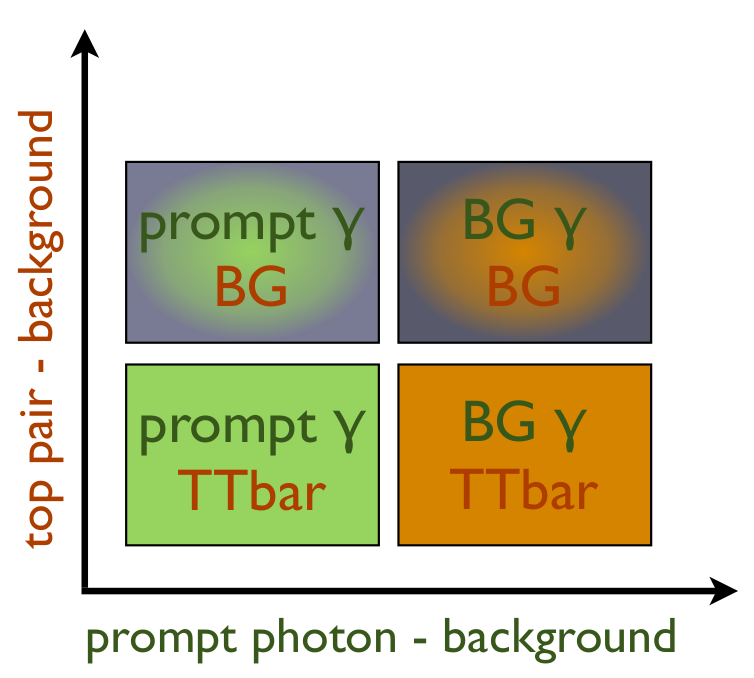
\includegraphics[scale=0.33]{Figures/SignalPhotonPlot.png}
\caption{Graphic representation of the signal and background definitions \cite{MishaSignalDefinition}.}
\end{center}
\end{figure}

\subsection{Background processes}

\begin{figure}\label{fig-AnalysisFlowChart}
\begin{center}
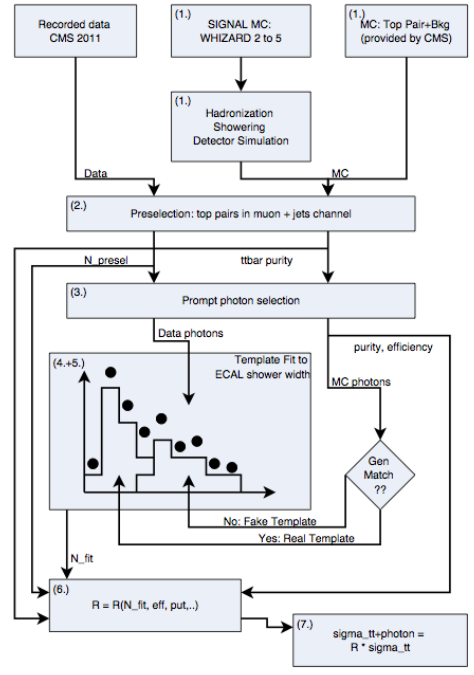
\includegraphics[width=0.75\textwidth]{Figures/AnalysisFlowChart.png}
\caption{Flow chart showing each stage of the analysis. The box numbers represent the outlined
analysis steps.}
\end{center}
\end{figure}

\section{$t\bar{t}+\gamma$ Signal Simulation}

WHIZARD

then

MADGRAPH

Factorised matrix element 

\section{Phase Space Overlap Removal} \label{sec-PhaseSpaceOverlapRemoval}

Events of the $t\bar{t}+\gamma$ process lie within a small region of $t\bar{t}$ phase space, and thus our signal sample events are expected to overlap with TTJets events in the case where a hard photon is radiated by initial state quarks, top quarks, b quarks, W and its decay products: electrons, muons, and their corresponding neutrino. In order to prevent the double counting of events we apply an overlap removal procedure to remove such events from our TTJets samples. In order for an event to be considered as overlapping with TTGamma, an event has to have at least one generator-level photon with the following properties:

\begin{itemize}
	\item p$_T(\gamma) > 13$ GeV
	\item $|\eta| < 3.0$
	\item Only gluons, bosons, or leptons are in the parents list. This ensures that photons from $\pi^0$ decays are not considered as signal
	\item $\Delta R(\gamma, other) > 0.2$ where other particles include leptons, b quarks and final state particles (hadrons, charged leptons, photons) with transverse momenta above $5 \GeV$.
\end{itemize}

The last cut is implemented in order to suppress photons from showers. In such cases the information from the parent particle will show that a photon is radiated by an electron, however the photon may be collinear with it. In particular in TTJets di-lepton events, such as described in this analysis, where a considerable fraction of the reconstructed photons comes from electrons radiating photons.

 Similarly, we also observe an overlap between Z+Jets and ZGamma processes, and between W+Jets and WGamma samples, for the same reasons as described above. The phase space overlap removal procedure is applied on Z+Jets and W+Jets samples to remove events containing generator-level photons. Events containing generated photons are removed in the case in which they are from initial state radiation (emitted from the colliding partons) or final state radiation (emitted from W or Z bosons or their decay products), since these are already included in the WGamma and ZGamma simulations. The overlap removal procedure removes approximately one percent of the events in the W+Jets sample, and approximately three to four percent of the events from the TTJets and Z+Jets samples.

\begin{figure} \label{fig-photonphasespace}
\begin{center}
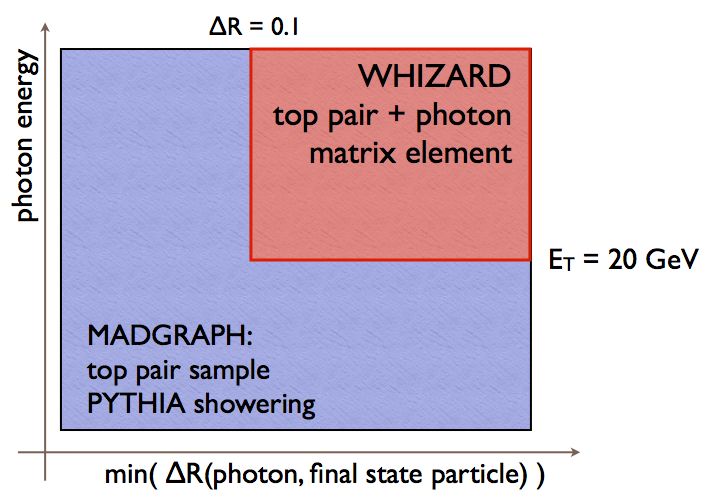
\includegraphics[scale=0.5]{Figures/photonphasespace.png}
\caption{}
\end{center}
\end{figure}

\section{Event Selection} \label{sec-EventSelection}

\section{Photon Purity Estimation} \label{sec-PhotonPurityEstimation}

\section{Signal Acceptance Calculation} \label{subsec-SignalAcceptanceCalculation}

Acceptance calculation for this analysis differs from usual inclusive cross section measurements because we measure ratio of cross sections. The event selection is chosen to make use of this fact: two steps (top selection and photon selection) are done sequentially. For the inclusive $t\bar{t}$ process, we start with number of generated events (within some fiducial phase space) and count how many events are left after top event selection. The acceptance times efficiency is defined for the $t\bar{t}$ top selection as:

\begin{equation}
	\epsilon^{t\bar{t}}_{top} \cdot A^{t\bar{t}}_{top} = \frac{N_{t\bar{t}.preselection}}{N_{t\bar{t}.generated}} 
\end{equation}

This gives the acceptance times efficiency of the inclusive $t\bar{t}$ process to be $\epsilon^{t\bar{t}}_{top} \cdot A^{t\bar{t}}_{top} =   \pm  (stat.)$ in the di-muon channel, $\epsilon^{t\bar{t}}_{top} \cdot A^{t\bar{t}}_{top} =  \pm  (stat.)$ in the di-electron channel, and $\epsilon^{t\bar{t}}_{top} \cdot A^{t\bar{t}}_{top} =  \pm  (stat.)$ in the mixed final state.

The same can be done for the $t\bar{t}+\gamma$ (signal sample). To get the acceptance times efficiency we have to divide the number of events passing top selection by the total number of events considered. However, in this case we have to choose what we take as the denominator. The signal $t\bar{t}+\gamma$ sample is inclusive, but theoretical calculations for the cross section are done for final states with 1 and 2 leptons \cite{QCDCorrectionsttgamma2011}. To make comparison with theory easier we consider the fiducial space for signal when 1 or 2 leptons are present. The $t\bar{t}+\gamma$ acceptance times efficiency of the top selection is defined for the signal samples with 1 or 2 leptons as:

\begin{equation}
	\epsilon^{t\bar{t}+\gamma}_{top} \cdot A^{t\bar{t}+\gamma}_{top} = \frac{N_{t\bar{t}+\gamma.preselection(1lor2l)}}{N_{t\bar{t}+\gamma.generated(1lor2l)}} 
\end{equation}

Giving the acceptance times efficiency of the inclusive $t\bar{t}+\gamma$ process to be $\epsilon^{t\bar{t}+\gamma}_{top} \cdot A^{t\bar{t}+\gamma}_{top} =   \pm  (stat.)$ in the di-muon channel, $\epsilon^{t\bar{t}+\gamma}_{top} \cdot A^{t\bar{t}+\gamma}_{top} =  \pm  (stat.)$ in the di-electron channel, and $\epsilon^{t\bar{t}+\gamma}_{top} \cdot A^{t\bar{t}+\gamma}_{top} =  \pm  (stat.)$ in the mixed final state.

The acceptance and efficiency for the $t\bar{t}+\gamma$ sample includes a term for photon selection. This is found based on the ratio of the number of events in $t\bar{t}+\gamma$ passing photon selection and the reconstructed photon matched to a generated photon over the number of events passing the top selection. The $t\bar{t}+\gamma$ photon selection acceptance times efficiency is defined as

\begin{equation}
	\epsilon^{t\bar{t}+\gamma}_{\gamma} \cdot A^{t\bar{t}+\gamma}_{\gamma} = \frac{N_{t\bar{t}+\gamma.photonselection(1lor2l)}}{N_{t\bar{t}+\gamma.preselection(1lor2l)}} 
\end{equation}

Thus, yields of the acceptance times efficiency of the inclusive $t\bar{t}+\gamma$ process to be $\epsilon^{t\bar{t}+\gamma}_{\gamma} \cdot A^{t\bar{t}+\gamma}_{\gamma} =   \pm  (stat.)$ in the di-muon channel, $\epsilon^{t\bar{t}+\gamma}_{\gamma} \cdot A^{t\bar{t}+\gamma}_{\gamma} =  \pm  (stat.)$ in the di-electron channel, and $\epsilon^{t\bar{t}+\gamma}_{\gamma} \cdot A^{t\bar{t}+\gamma}_{\gamma} =  \pm  (stat.)$ in the mixed final state.

The calculation of signal acceptance explained above is done for the sake of comparison with theoretical prediction. The biggest difference in the generated phase space and analysis selection is the transverse energy cut on the photon (13 GeV in generated sample and 25 GeV in analysis). We are measuring the value for the higher $E_T$ cut on the photon and using the efficiencies to extrapolate back to the full generated phase space. In order to avoid this propagation of the result into the larger phase space we also quote the \emph{visible cross section ratio}, where the cross section is measured in the fiducial region with generated photons having transverse energy of at least 25 GeV and $| \eta | < 1.4442$. For the visible cross section ratio, the photon selection term includes only the photon reconstruction efficiency because, by definition, we are considering events where generator photon passes analysis level $p_T$ and $\eta$ cuts.

The visible top selection efficiency in $t\bar{t}+\gamma$ is taken to be the ratio of the number of $t\bar{t}+\gamma$ events passing the preselection (with a generated photon having $p_T > 25$ GeV and $| \eta | < 1.4442)$

\begin{equation}
	\epsilon^{t\bar{t}+\gamma Vis}_{top} = \frac{N_{t\bar{t}+\gamma.preselection(1lor2l)}\left( p_T(\gamma_{gen}) > 25 GeV, |\eta(\gamma^{gen})| < 1.4442 \right)}{N_{t\bar{t}+\gamma.generated(1lor2l)}\left( p_T(\gamma_{gen}) > 25 GeV, |\eta(\gamma^{gen})| < 1.4442 \right)} 
\end{equation}

The $t\bar{t}+\gamma$ visible photon selection efficiency is calculated as the ratio of $t\bar{t}+\gamma$ events passing to photon selection with a reconstructed photon matched to a generated photon over the number of events passing top selection and with an isolated generator level photon passing the $p_T > 25$ GeV and $| \eta | < 1.4442$ cuts used in the photon selection.

\begin{equation}
	\epsilon^{t\bar{t}+\gamma Vis}_{\gamma} = \frac{N_{t\bar{t}+\gamma.photonselection(1lor2l)}\left( p_T(\gamma_{gen}) > 25 GeV, |\eta(\gamma^{gen})| < 1.4442 \right)}{N_{t\bar{t}+\gamma.preselection(1lor2l)}\left( p_T(\gamma_{gen}) > 25 GeV, |\eta(\gamma^{gen})| < 1.4442 \right)} 
\end{equation}

The visible top selection efficiency is found to be $\epsilon^{t\bar{t}+\gamma Vis}_{top} = 0.0712 \pm 0.0005$, $\epsilon^{t\bar{t}+\gamma Vis}_{\gamma} = 0.0928 \pm 0.0006$, and $\epsilon^{t\bar{t}+\gamma Vis}_{\gamma}$ in the di-muon, di-electron and mixed channels, respectively. The value of the visible photon selection efficiency is found to be $\epsilon^{t\bar{t}+\gamma Vis}_{\gamma} = 0.287 \pm 0.004 ( stat.)$ for the di-muon final state, $\epsilon^{t\bar{t}+\gamma Vis}_{\gamma} = 0.286 ± 0.004 (stat.)$ for the di-electron channel, and $\epsilon^{t\bar{t}+\gamma Vis}_{\gamma} = 0.287 \pm 0.004 ( stat.)$ for the mixed final state.

\chapter{Measurement of the anomalous couplings of the photon to the top quark}\label{chap-anomolouscouplings}

\chapter{Electron Conversion Veto}\label{chap-conversionveto}


\chapter*{Conclusions}\label{chap-conclusions}

In this thesis we present the observation and cross-section measurement of top quark pairs in association with a radiated photon decaying to a dilepton final state. The measurement was made using data from proton-proton collisions recorded by the CMS detector at the Large Hadron Collider, running with a centre-of-mass energy of $\sqrt{s} = 8$ TeV over the 2012 data-taking period. 

A cut-based analysis measuring the production cross-section of top quark pair events in association of a radiated photon, as well as the ratio of the production cross-section to the inclusive top quark pair cross-section, was carried out using the full 2012 dataset corresponding to an integrated luminosity of $19.7$ fb$^{-1}$. We take the ratio of cross-sections in order to cancel out global variables, such as luminosity. The estimation of the photon identification efficiency is calculated by studying the photon isolation profile using the supercluster footprint removal technique and random cone isolation. This method allows us to extract signal and background templates directly from data. The technique is cross-checked with simulated events for completeness. 

The main sources of uncertainty for the measurement manifest in the form of the purity of top pair events passing selection, and the number of photon events passing full selection. The precision of the cross-section calculation is limited due to the very small number of events passing selection. A cross-section of $\sigma_{t\bar{t}+\gamma} = 983 \pm 32$ fb and ratio $R = \sigma_{t\bar{t}+\gamma}/\sigma_{t\bar{t}} = 0.00221 \pm 0.00023$ was measured in comparison to the theoretical prediction of $\sigma_{t\bar{t}+\gamma}^{theoretical} = 861 \pm 182$ fb, using the latest measurement of the inclusive $t\bar{t}$ cross-section. Therefore, we observe a good agreement with the Standard Model and do not observe any evidence for physics beyond that of the Standard Model. This is the most accurate measurement of the $t\bar{t}+\gamma$ process to date and the only measurement in the dilepton final state ever performed.  


\section{Future Outlook}

Overall, the outlook for a measurement of the $t\bar{t}+\gamma$ process at higher energies is an exciting prospect. It will be possible to measure the cross-section of the process to a much higher degree of accuracy due to the increase in the production of top quark pairs compared to a much lower production rate of background processes. For an LHC running at centre-of-mass energy of $\sqrt{s} = 14$ TeV, we expect a cross-section for top quark pairs to have increased by $\sim3.5$ times the cross-section at $\sqrt{s} = 8$ TeV at $920$ pb \cite{Czakon:2013goa}, compared to an increase of $\sim1.5$ times that at $\sqrt{s} = 8$ TeV for background processes. This can be seen in Figure \ref{fig-ttbarXsectPlot}. This increase in top quark pair production would remove the main inhibitor of the measurement -- it is statistically limited.

Ultimately, we would like to measure the electromagnetic vertex of the top quark and radiated photon, however it could also be used in conjunction with other measurements. For example, a future $t\bar{t}+\gamma$ measurement could also be used in a way that is complementary to the search for top quark pair plus a radiated Higgs boson, whereby the Higgs decays to two photons in the final state. Understanding this process will be of huge importance as it will be a background to the $t\bar{t}+\gamma$ process, and a combination of semileptonic and dileptonic channels would be more beneficial at higher energies due to increased statistics. Similarly, understanding the $t\bar{t}+\gamma$ process is greatly import as it is a background to many SUSY processes. At higher energies it will be possible to glean a greater understanding of the process by measuring the differential cross-section with respect to global variables. 

\addcontentsline{toc}{chapter}{Conclusions}

\appendix
\appendixpage
\addappheadtotoc

\renewcommand{\thesection}{A.\arabic{section}}
\renewcommand\thefigure{\thesection}
\renewcommand\thetable{\thesection}

\bibliography{PhDThesis}
\bibliographystyle{unsrt}

\end{document}
